\documentclass[11pt]{book}

\usepackage{fullpage}
\usepackage{graphicx}
\usepackage{cite}
\usepackage{times}
\usepackage{url}
\usepackage{setspace}
\usepackage{fancyhdr}
\usepackage{ifthen}
\usepackage{listings}
\usepackage[section]{placeins}
\usepackage{xtab}
\usepackage{url}

\setcounter{topnumber}{2}
\setcounter{bottomnumber}{3}
\setcounter{totalnumber}{4}  
\renewcommand{\topfraction}{0.5}
\renewcommand{\bottomfraction}{0.95}
\renewcommand{\textfraction}{0.1}
\renewcommand{\floatpagefraction}{0.7}

\setlength{\abovecaptionskip}{3pt}
\setlength{\belowcaptionskip}{3pt}

\pagestyle{fancy}
\setboolean{@twoside}{false} 
\setlength{\headsep}{25pt}
\setlength{\headheight}{14pt}

\begin{document}

\thispagestyle{empty}

\doublespacing

\vspace*{0.5in}

\begin{center}
\LARGE{\textbf{Put your thesis title here}}

\vspace*{0.4in}

  {\large A thesis submitted to the\\[0.20in]
    Division of Research and Advanced Studies\\
    of the University of Cincinnati\\[0.20in]
    in partial fulfillment of the\\
    requirements for the degree of\\[0.20in]
    {\bf MASTER OF SCIENCE}\\[0.20in]
    in the School of Electric and Computing Systems\\
    of the College of Engineering and Applied Sciences\\[0.20in]
    August xx, 2010\\[0.20in]
    by\\[0.20in]
    {\bf Your Name Here}\\
    BSxx, University of Someplace, 20xx\\}
  \vspace{0.5in}
  {\large Thesis Advisor and Committee Chair:  Dr. Philip A. Wilsey}
\end{center}

\clearpage

\setcounter{page}{1}
\pagenumbering{roman}
\clearpage

\chapter*{Abstract} 




\tableofcontents \markright{ }
\listoffigures \markright{ }
\listoftables \markright{ }

\clearpage
\pagenumbering{arabic} \setcounter{page}{1}

\chapter{Introduction}\label{intro} 

The potential performance improvement of distributing a computation over a number of parallel nodes is frequently determined by the amount of network communication necessary. The time required to send a single message between computers on a local network can be on the order of milliseconds, while modern processors can execute an instruction in much less than a nanosecond. Therefore, the run time of a computation that requires a large amount of communication can be dominated by the costs of sending network messages.  Discrete Event Simulation (DES) is one such fine grained computation.

The primary task of a DES is to send events between simulation objects. For models in which the processing requirements for a single event is low, the simulation can be almost entirely composed of message passing. In a sequential DES, sending an event between objects requires, at most, a memory copy. In a Parallel Discrete Event Simulation (PDES), sending an event may require that event data be serialized into a network message. For certain simulation models (workloads), this means that nearly the entire simulation time is spend sending network messages. 

This thesis presents a method of reducing simulation network traffic in PDES simulations while balancing processor load by using data collected from profiling to perform partitioning of simulation objects between processors, with the goal of reducing overall simulation time. The effectiveness of this method is demonstrated by implementing profile guided partitioning in the \texttt{WARPED} PDES Kernel. The message passing characteristics of a number of real world models are profiled, then the collected data is used to perform partitioning. This performance of this implementation evaluated against a naive partitioning algorithm.

\section{Principle Hypothesis}

The principle hypothesis of this thesis is that the overhead of sending events between nodes in a PDES simulation has a large impact on its runtime, and that profile guided partitioning can significantly reduce the amount of events sent between nodes, thereby improving simulation performance. This thesis explores the event passing characteristics and performance of a number of real world models run in a Time Warp simulator.

\section{Thesis Overview}

The remainder of this thesis is organized as follows:
 
Chapter \ref{background}

Chapter \ref{relatedWork}


Finally, Chapter \ref{conclude}


\chapter{Background}\label{background}

This chapter introduces the concepts central to this thesis. Information on general Discrete Event Simulation (DES) is given, followed by information on Parallel Discrete Event Simulation (PDES), and finally by information on the Time Warp architecture and the WARPED simulator.

\subsection{Discrete Event Simulation}

A Discrete Event Simulation primarily deals with sending events between objects. The term \emph{simulation object} refers to a single object in the simulation. Each simulation object may have a collection of state that changes in response to \emph{events}. Events are messages sent between objects, and can contain data provided by the object that created them. Each event also carries a timestamp that defines when the event should be executed. An object may generate 0, 1, or multiple output events in response to an input event. 

For example, in the case of a digital circuit model, the objects are the gates, and the events are logic signals sent between connected gates. The simulation is not concerned with the physical propagation of the electrical signals across wires. When the output of a gate changes, the simulator calculates the propagation time of the signal, then adds the event to a priority queue that is sorted on the timestamp of events. This queue is often referred to as a Least Time Stamp First queue, or LTSF queue. The simulator then pops an event off of the LTSF queue and fast forwards its simulation clock to the timestamp of that event. The simulator then sends the event to its target object, which calculates its new output and sends events to any connected object. This process repeats until there are no more event exists to be processed, or until a preset simulation time has been reached.

\subsection{Parallel Discrete Event Simulation}

It is often desirable to attempt to increase performance of a sequential Discrete Event Simulation by distributing the workload across multiple processes (often called \emph{nodes}) that can execute in parallel. In a Parallel Discrete Event Simulation (PDES), the set of simulation objects is partitioned into disjoint subsets. Each partition of objects is assigned to its own \emph{logical process} (LP) that executes independently. All LPs are able to execute concurrently, processing events destined for the objects they contain. 

The parallel approach to DES brings with it a number of challenges. As with any concurrent computation, synchronization is an issue. Because each LP runs at a different speed, it is possible that the simulation times of the LPs will diverge. When this happens, an event with a larger timestamp may be executed before an event with a lower, violating causality of the simulation. There are two main synchronization approaches to preventing causality violations in PDES: \emph{Conservative Synchronization} and \emph{Optimistic Synchronization} \cite{fujimoto-90}.

Conservative Synchronization avoid the possibility of causality errors by synchronizing all LPs such that an event is not processed by any LP until all events that may affect it have been processed. If an LP has no events that can be processed safely without potentially violating causality, the process blocks until it is safe to process the event. This is straight forward, but blocking processes wastes processing time, and may lead to deadlocks if a cycle of LP are waiting on each other in a way that prevents any of them from proceeding. Additionally, since no LP can process an event that can violate causality, the entire simulation can only proceed as quickly as the slowest LP, which is referred to as the \emph{critical path}.

Optimistic Synchronization takes a very different approach, in that it does not attempt to prevent causality violations. Instead, causality errors are detected and the simulation is rolled back to undo the errors. Time Warp is one of the most well-known architectures for Optimistic Synchronization of PDES. In a Time Warp simulator, each LP copies that state of its objects at regular intervals called \emph{checkpoints}, and runs at full speed, as if it will never receive an event that would cause a causality error. If a LP detects that a causality violation has occurred (i.e., it receives an event with a timestamp lower than an event it has already processed), it rolls back the state of its internal objects to a checkpoint before the timestamp of the received event. If the LP performing the rollback had sent any events that need to be rolled back to other LPs, it then send messages (termed \emph{Anti-Messages}) that inform the LPs of the invalid events. This allows all LPs in the simulation to run at full speed, which in turn allows for the possibility that the simulation can run faster than the critical path. 

Each LP in a Time Warp synchronized PDES has its own Local Virtual Time (LVT). This is the timestamp of the most recently processed event. The Global Virtual Time (GVT) is lowest timestamp of any unprocessed event in the simulation. Because no events with a timestamp lower than the GVT will ever by processed, it is safe for the simulator to free memory used  by events or saved states with lower timestamps.

\subsection{The WARPED PDES Simulator}

The work for this thesis was built on an existing PDES simulator, the WARPED simulation kernel. WARPED was developed at the University of Cincinnati and is a C++ implementation of Time Warp \cite{king-10}.  WARPED is designed in an object oriented fashion, and uses inheritance for modularity. It is built around the concept of “managers” that control various components of the simulation. 

The core of the library are the \texttt{SimulationManager} classes, which are analogues to a LP. They own other simulation components and coordinate their functionality. WARPED can be configured at runtime to select from various subclasses of the \texttt{SimulationManager}, including the \texttt{SequentialSimulationManager}, which, as the name suggests, will run the simulation sequentially on a single process. Another option is the \texttt{TimeWarpSimulationManager}, which is used to run the Time Warp synchronized, distributed simulation. 

New simulation models are written by inheriting from the \texttt{Application} class, which is responsible for allocating the objects for the simulation in the form of subclasses of the \texttt{SimualtionObject} class. Prior to the work done for this thesis, these objects would be allocated by filling a \texttt{PartitionInfo} object, which would describe the partitions that would be used in the simulation. This approach was modified to allow for run-time configurable partitioning. These modifications are described in later chapters.

\subsection{Partitioning and Load Balancing}

...

\chapter{Related Work}\label{relatedWork}


\chapter{Overview of the Approach}\label{overview}

This chapter will provide an overview of the approach taken to implement Profile Guided Partitioning in the WARPED Simulator. In the first section, a description of a simulation model written for this thesis will be given. This model will be used as an example in the second section, which describes profiling WARPED models, and using the gathered information to perform partitioning. 

\subsection{The ISCAS’89 Simulation Model}

In 1989, the International Symposium on Circuits and Systems released a set of digital circuit descriptions named the ISCAS’89 Benchmarks. These circuits have been widely used as a standard set of circuits to study VLSI systems and simulators. The benchmark consists a number of circuits of varying sizes and complexities. Each circuit description is a list of components including inputs, outputs, logic gates (AND, NOT, NOR, etc.), and D Flip-Flops. The connections for all components are given, with many logic gates having more than two inputs. For this thesis, three of the ISCAS’89 circuits are studied: s5378, s9234, and s38584.1. Although high-level descriptions for most ISCAS’89 circuits do not exist, statistics on the components of each circuits can be found in Table~\ref{table:iscasStats}.

\subsection{Profiling WARPED Models}

Although there are a number of aspects of a simulation that could be profiled, the count of events sent between objects is the statistic used in this thesis. This was chosen over other possible statistics because it is a direct measure of the amount of network traffic that will be generated in distributed simulation. Additionally, the event count characteristic of the model and inputs, and is independent of the method of simulation or the platform on which the simulation is run. Profiling an aspect such as the number of rollbacks only works on a time warp simulator and is highly dependent on the system the simulation is run on. Running several identical simulations on the same platform will result in widely varying numbers or rollbacks.

The statistics gathered on a model can be represented by an undirected graph \(G = (V, E)\), comprising the set \(V\) of vertices and the set \(E\) of edges. For each simulation object \(o_i\), there exists exactly one vertex \(v_i \in V\). An edge \(e_{i,j} \in E\)  indicates that at least one event was sent from \(o_i\) to \(o_j\) during the simulation, or from \(o_j\) to \(o_i\), without regard to the direction the event was sent. The graph can then be weighted with the collected statistics. The weight assigned to edge \(e_{i,j}\) is the total number of events sent between \(o_i\) and \(o_j\). 

A graph statistics collected on the s9234 ISCAS’89 model can be seen in Figure~\ref{fig:iscasUnpart}. This figure represents the weight of the edges as a heat map, with thick, red edges corresponding to heavily weighted edges, and thin, blue or green edges corresponding to lightly weighted edges. For this model, the most heavily weighted edges had a weight several orders of magnitude larger than the average edge, as can be seen in figure~\ref{fig:s9234_histo}. This model clearly exhibits the power-law behavior that is common in real-world models \cite{clauset-09}.

\subsection{Profile Guided Partitioning}

\chapter{Implementation Details}\label{detailedImplementation}

This chapter describes the details of the implementation of Profile Guided Partitioning in the WARPED kernel. In the first section, the method used to collect statistics is detailed. Next, the choice of partitioning library is described and the modifications to the WARPED kernel required for run-time configurable partitioning are detailed.

The approach taken was a two-step process. Profile data is collected during a sequential simulation run and stored in an intermediate file on disk. This statistics file is then read by WARPED when run in a parallel configuration in order to perform partitioning. It would be possible to perform profiling automatically in one step, which would save a small amount of user intervention, but there are a number of drawback to automatic partitioning that led to the choice of the current procedure.

Firstly, profiling takes time. By saving the results to disk a user is able to perform profiling once, then use the collected data for multiple runs. Because the profiling data is independent of the platform used, including the number of simulation nodes, a benchmarking run consisting of multiple system configurations only needs to perform profiling once. 

Of course, it would be possible to cache the profiling results between simulation runs, even if the profiling was performed automatically. However, the one-step process still has a larger drawback. Some simulation models have a natural termination condition. For example, a VLSI circuit model might read in a fixed-length input vector and terminate once all inputs have propagated through the circuit. Not all models terminate naturally, however. A model of disease epidemic spreading through a geographic area may not have a natural termination condition. Instead, this model would run until a given GVT value was reached. Even if a model does have a natural termination condition, it may be a very long running simulation. In this case, it is desirable to terminate at a given GVT to save time. Either way, an automated one-step profiling procedure would not be able to automatically determine the termination settings. Because of this, the two-step process in advantageous.

\subsection{Collecting Profiling Data}
...
\subsection{Run-Time Configurable Partitioning}
...
\subsection{Partitioning with METIS}
...

\chapter{Performance Analysis}\label{analysis}


\chapter{Summary of Results}\label{resultsSummary}

\chapter[Conclusions \& Future Research]{Conclusions and Suggestions for Future Research}\label{conclude}

\section{Summary of Findings}

\section{Detailed Conclusions}

\section{Suggestions for Future Work}


\appendix
\chapter{Appendix A}\label{appendixA}

\begin{figure}
\centering
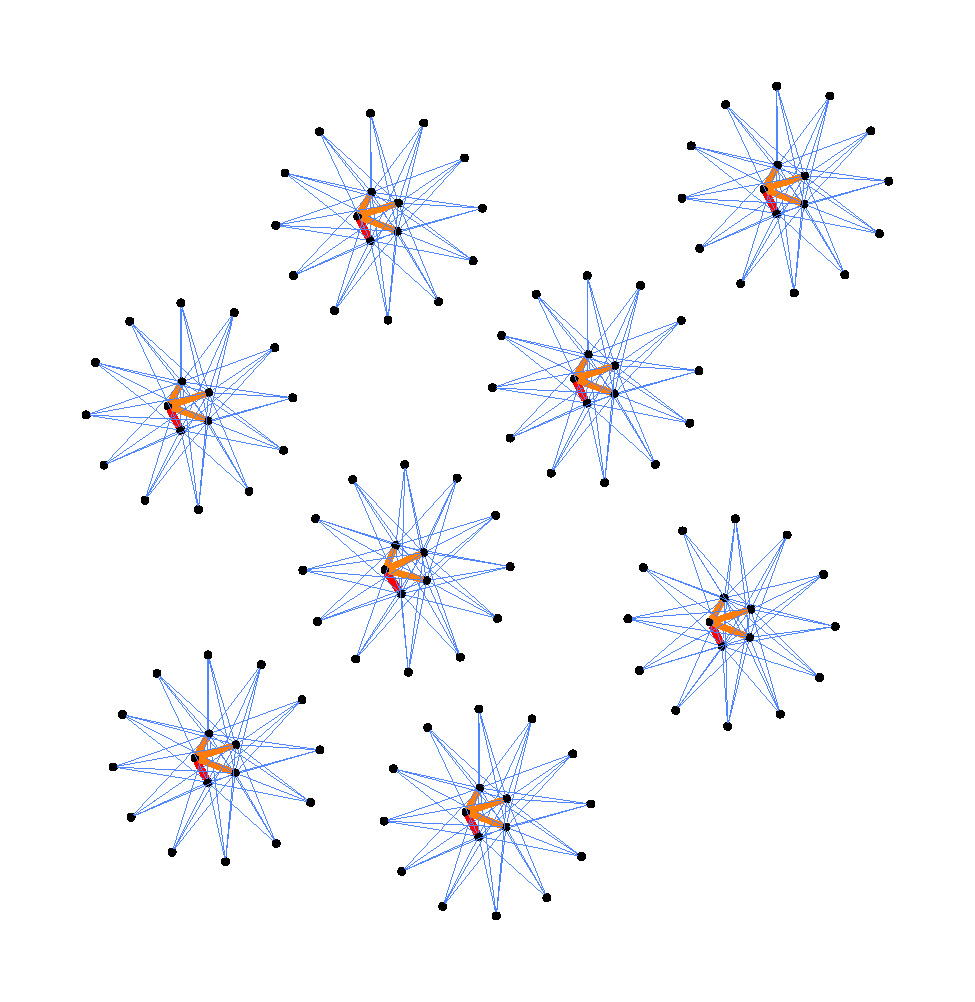
\includegraphics[clip=true,width=0.5\textwidth]{figs/RAID.pdf}
\caption{Heatmap of messages sent during the RAID simulation.}
\end{figure}

\begin{figure}
\centering
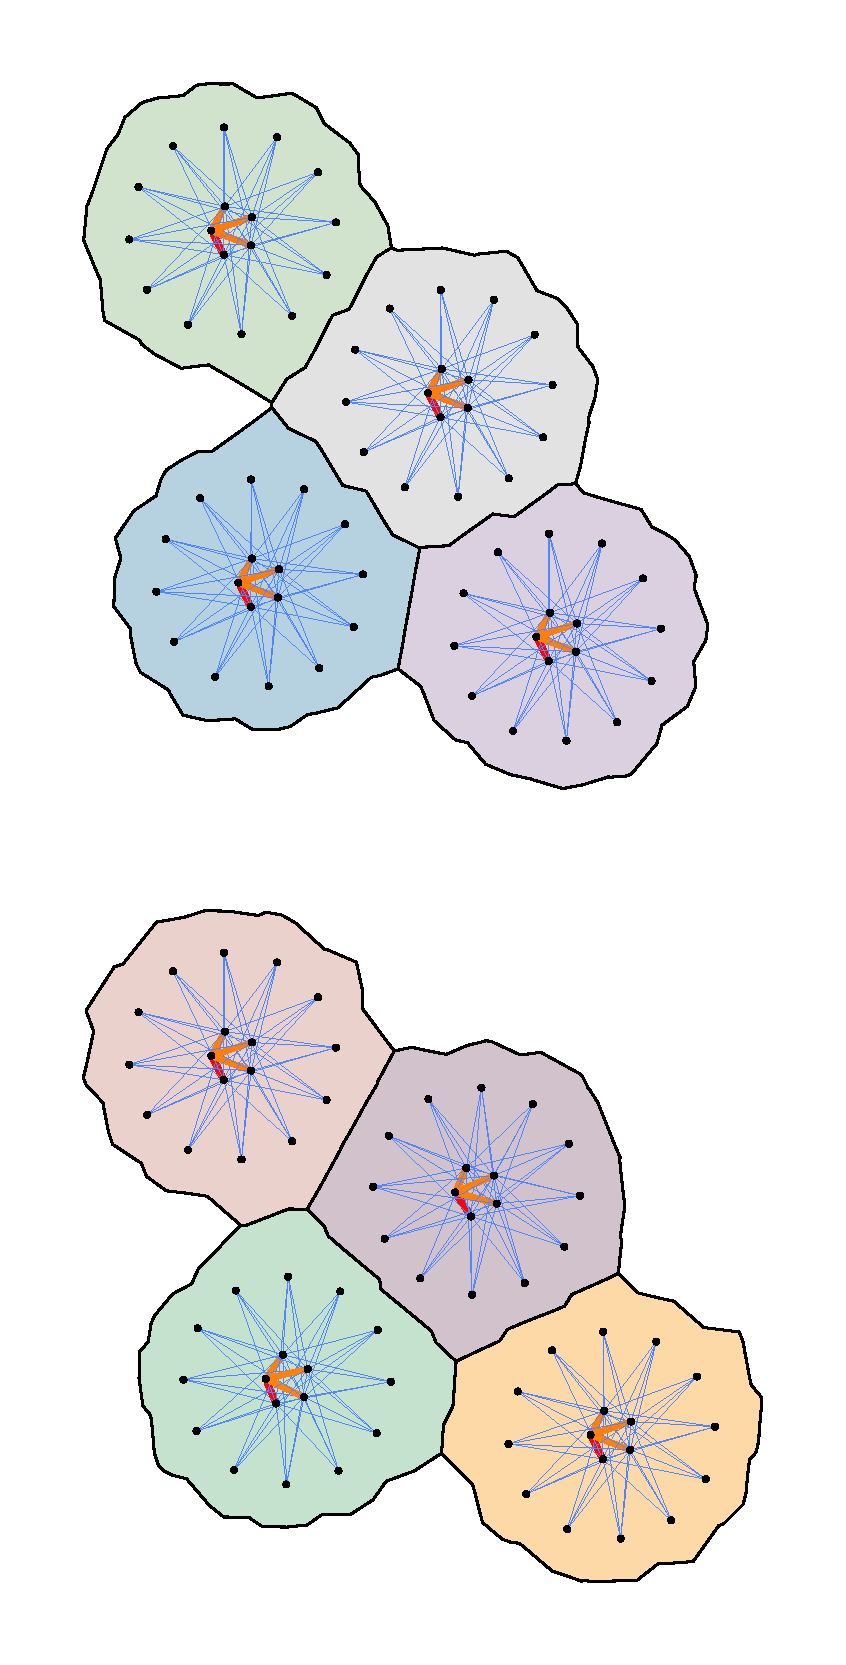
\includegraphics[clip=true,width=0.5\textwidth]{figs/RAID_2part.pdf}
\caption{Heatmap of messages sent during the RAID simulation, partitioned into two partitions using the profile guided algorithm.}
\end{figure}

\begin{figure}
\centering
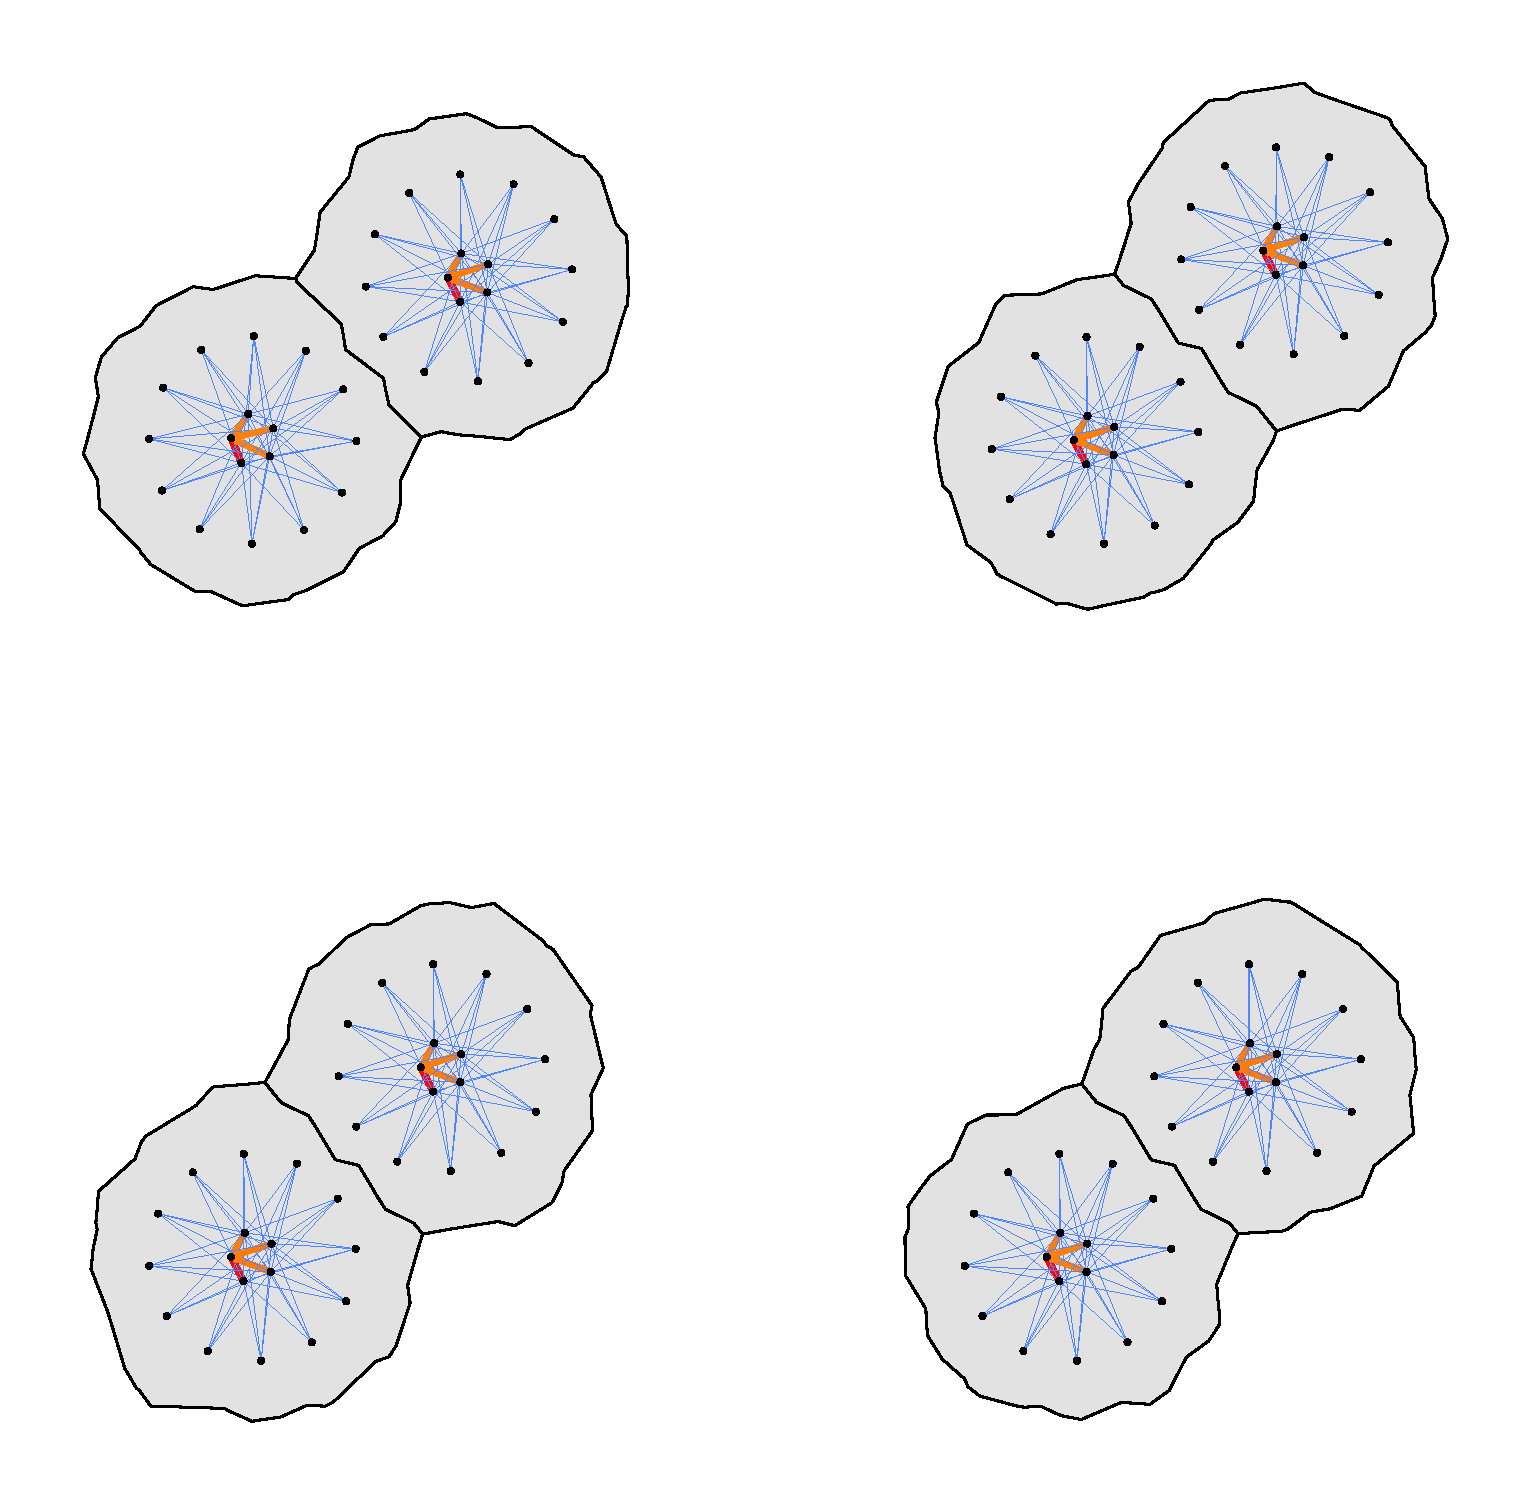
\includegraphics[clip=true,width=0.5\textwidth]{figs/RAID_4part.pdf}
\caption{Heatmap of messages sent during the RAID simulation, partitioned into four partitions using the profile guided algorithm.}
\end{figure}

\begin{figure}
\centering
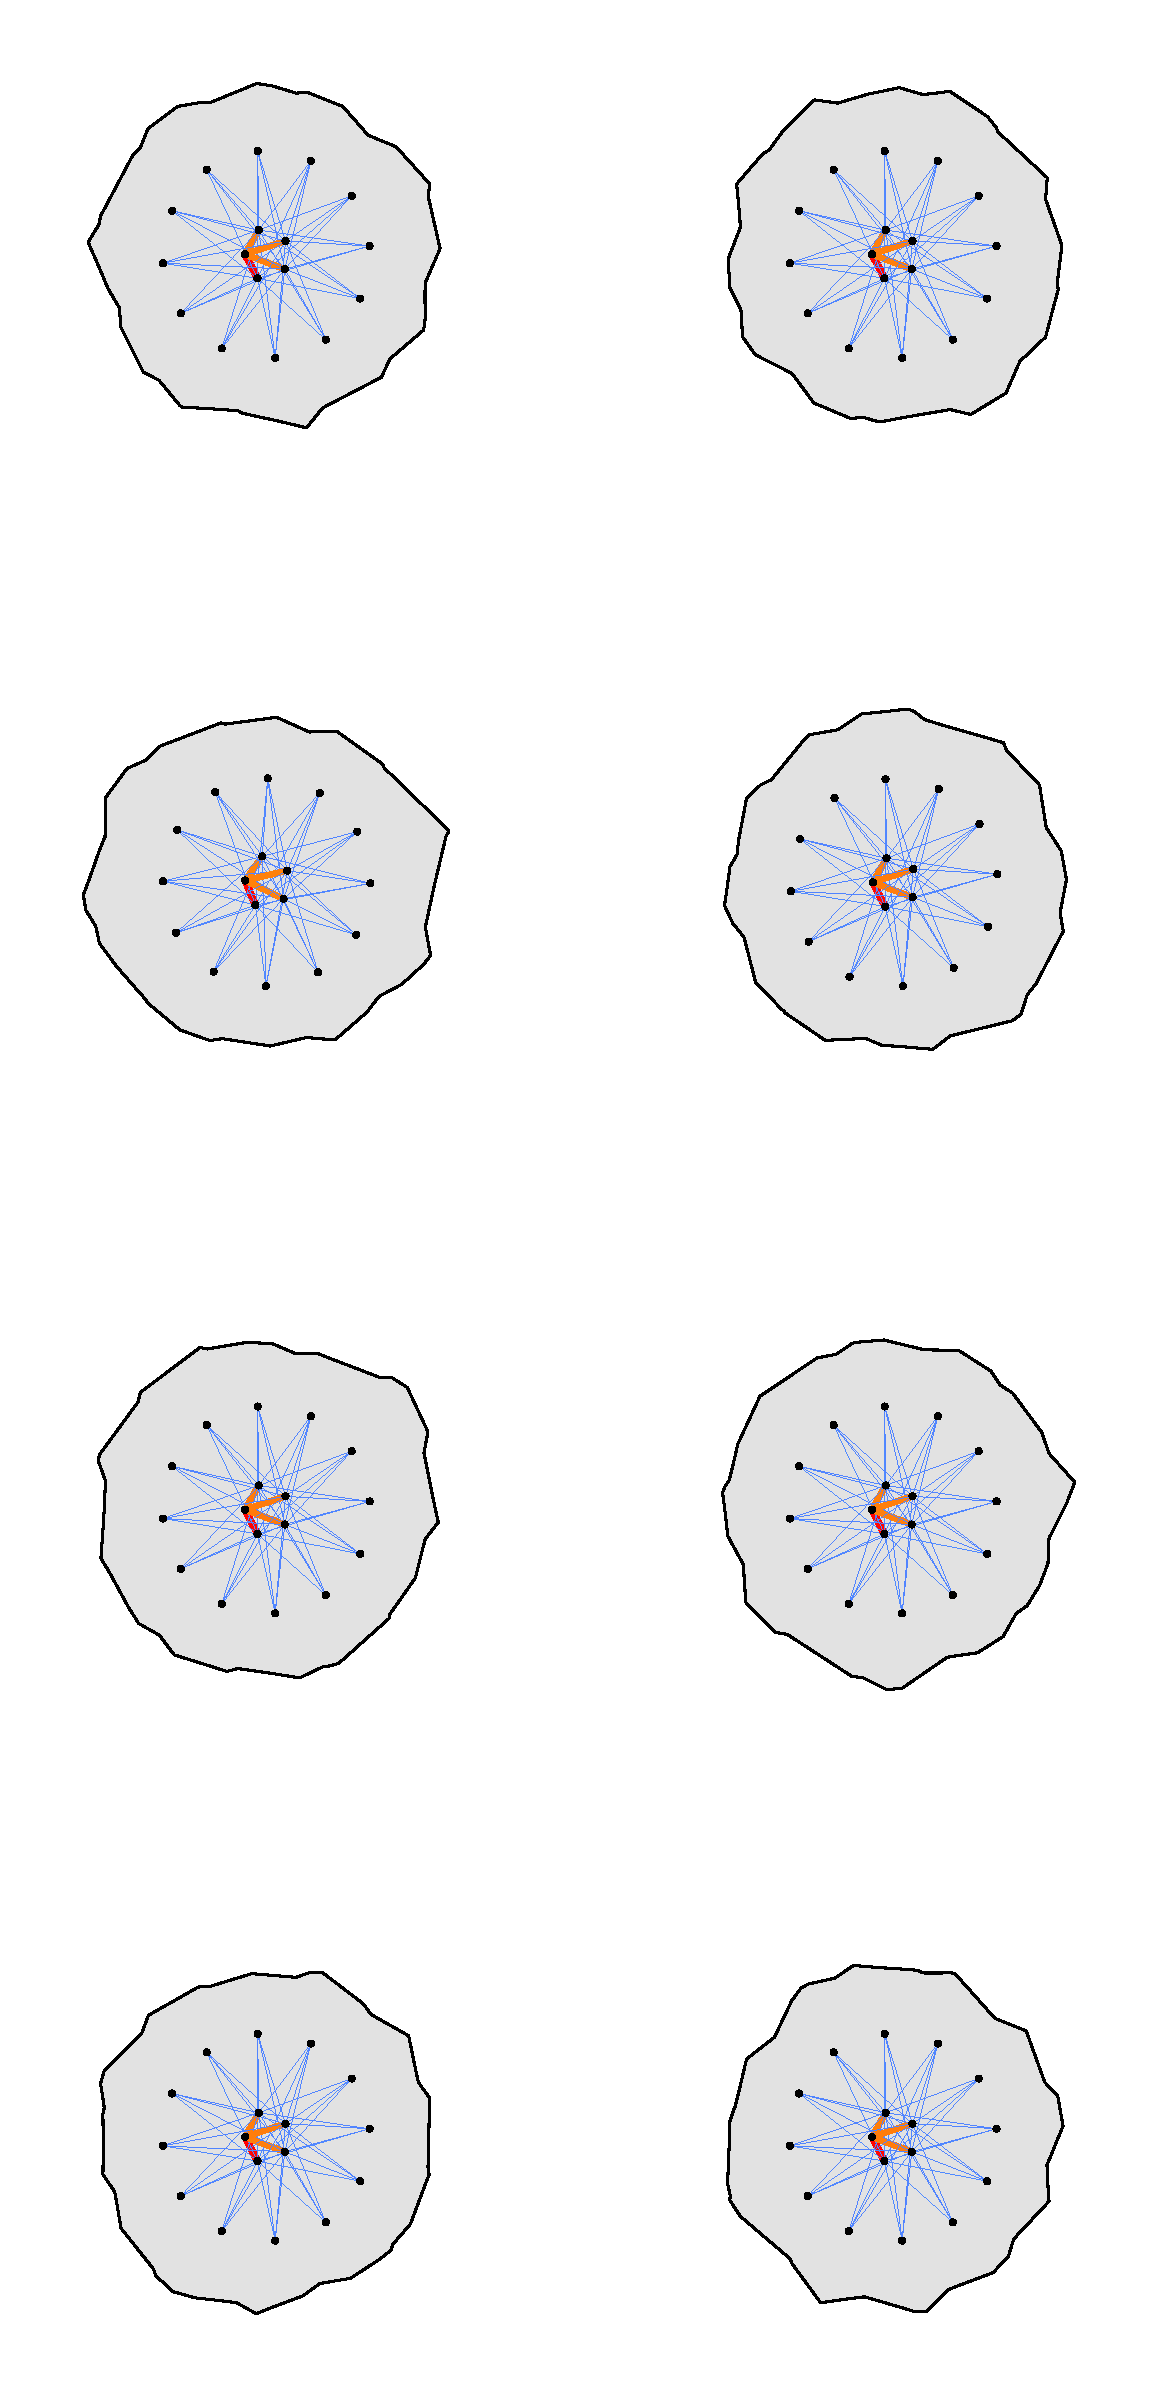
\includegraphics[clip=true,width=0.5\textwidth]{figs/RAID_8part.pdf}
\caption{Heatmap of messages sent during the RAID simulation, partitioned into eight partitions using the profile guided algorithm.}
\end{figure}

\begin{figure}
\centering
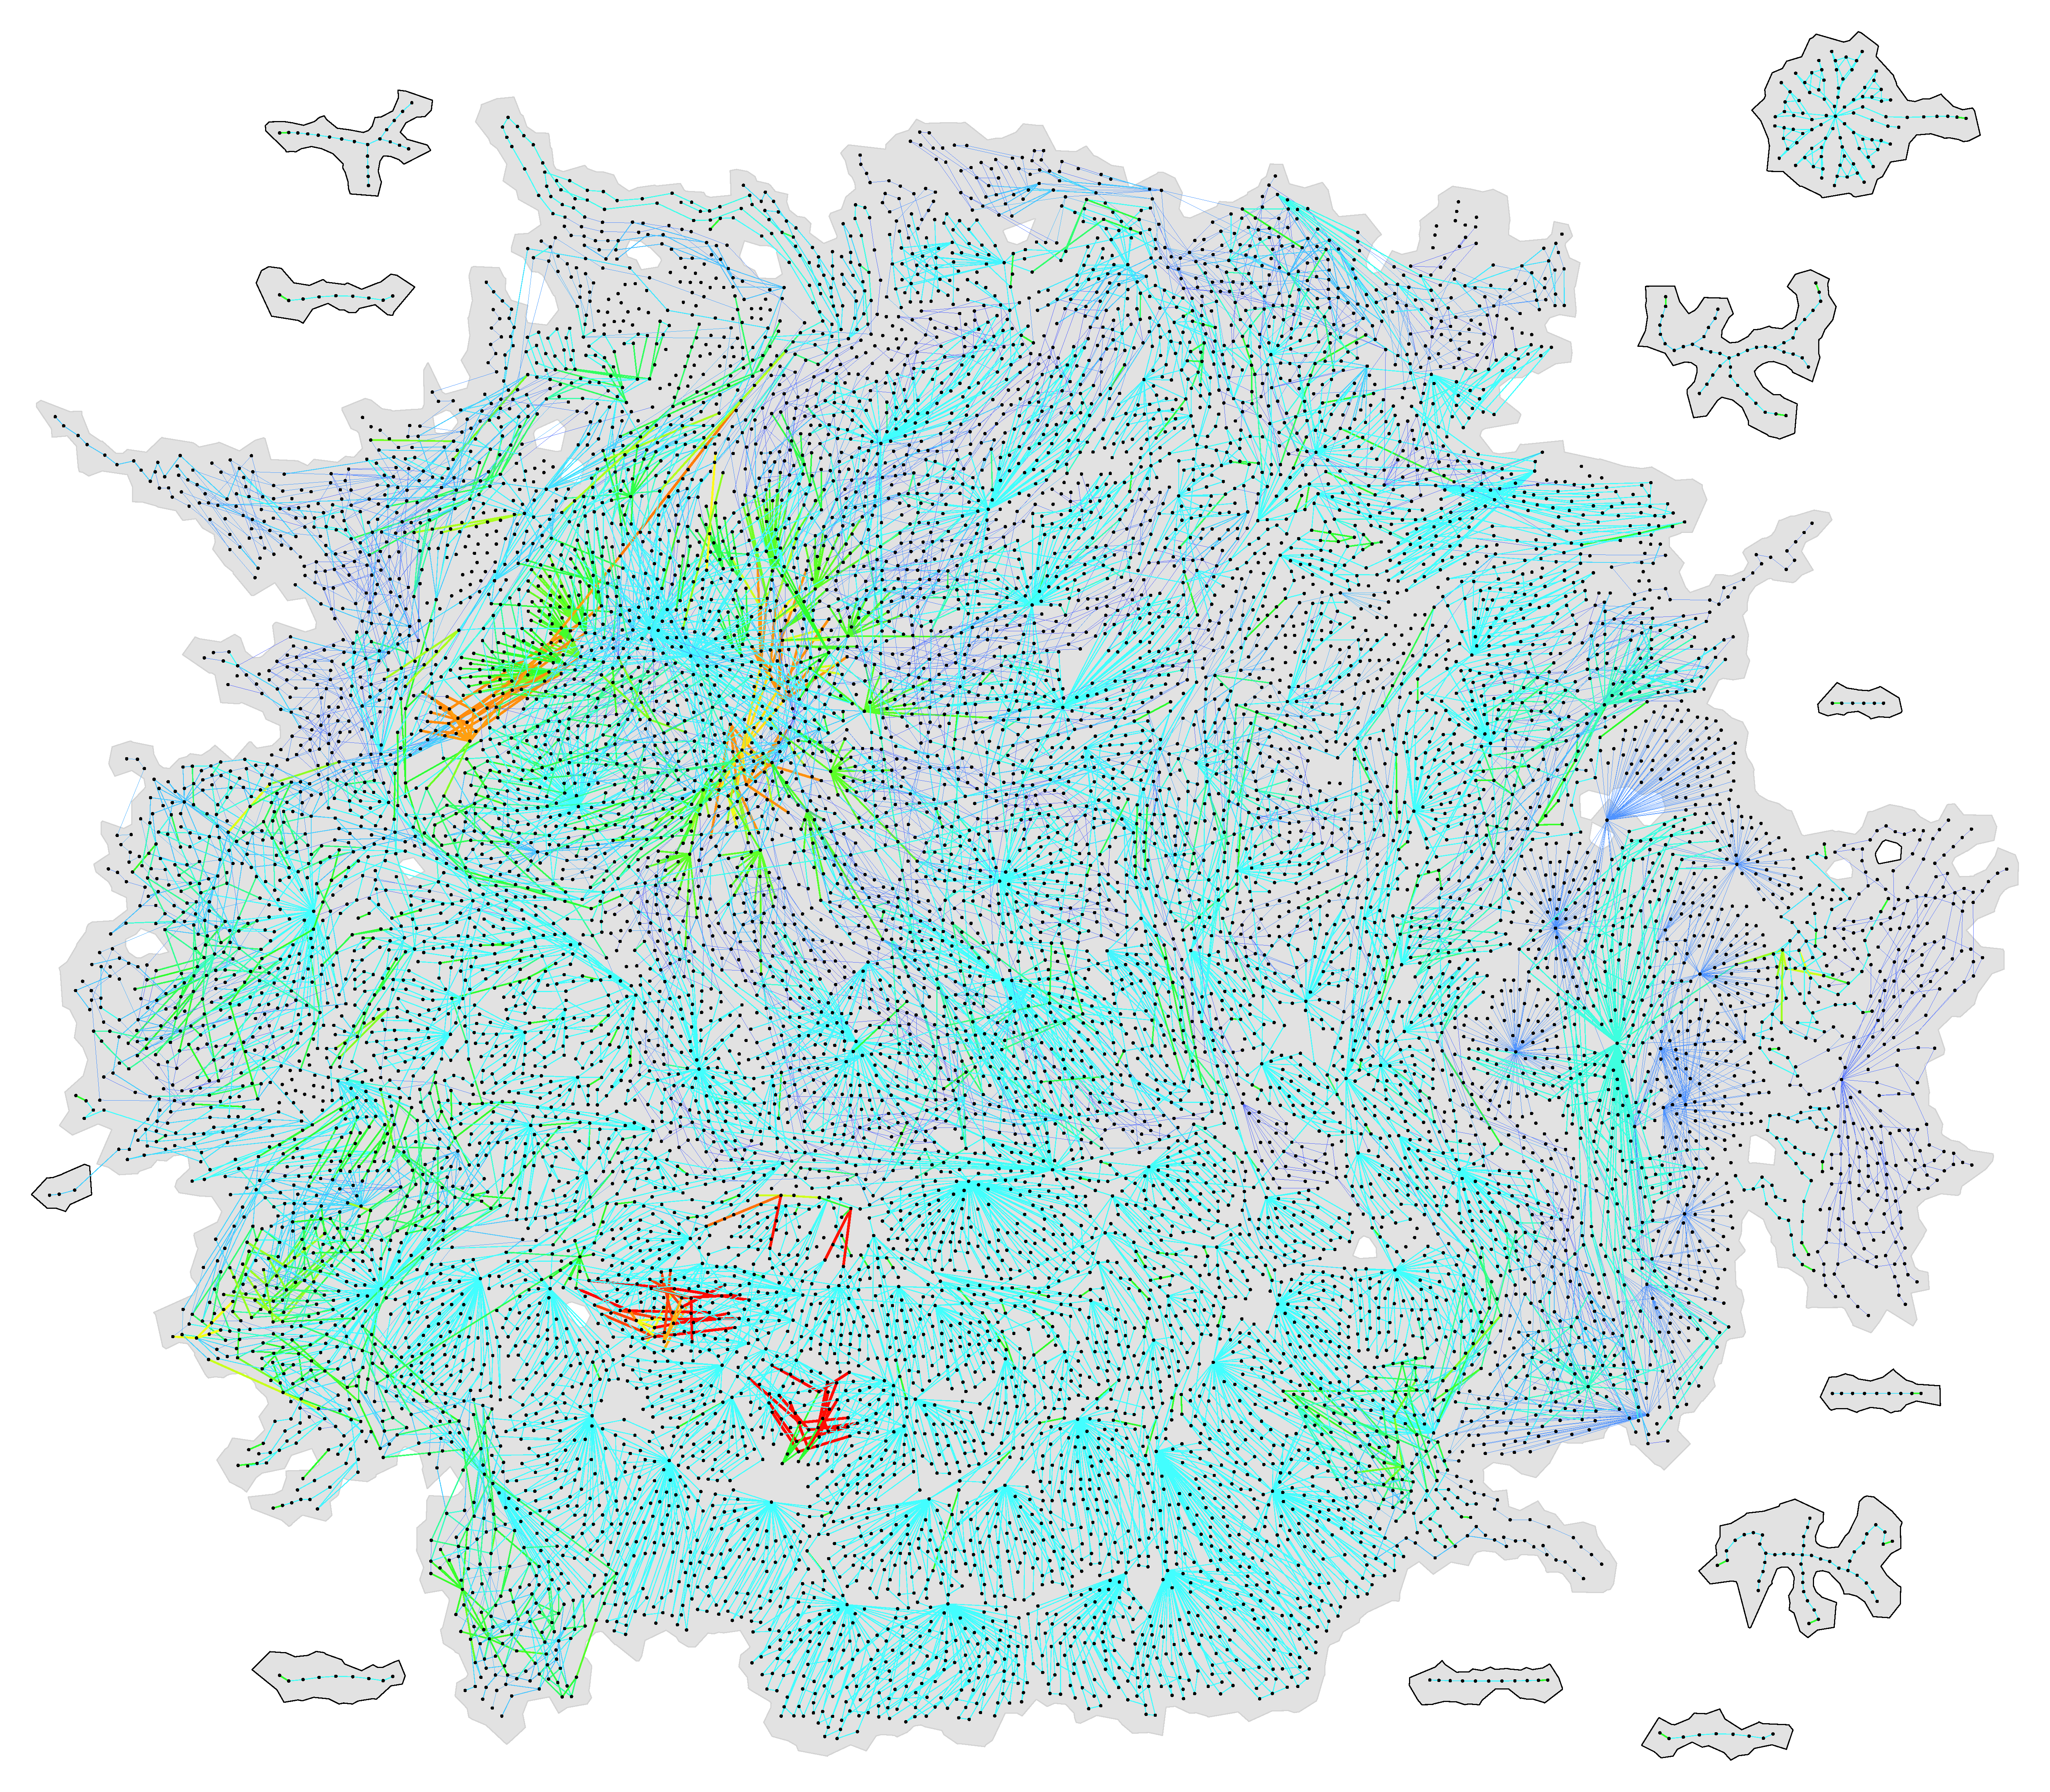
\includegraphics[clip=true,width=0.5\textwidth]{figs/s38584.pdf}
\caption{Heatmap of messages sent during the ISCAS'89 s38584 simulation.}
\end{figure}

\begin{figure}
\centering
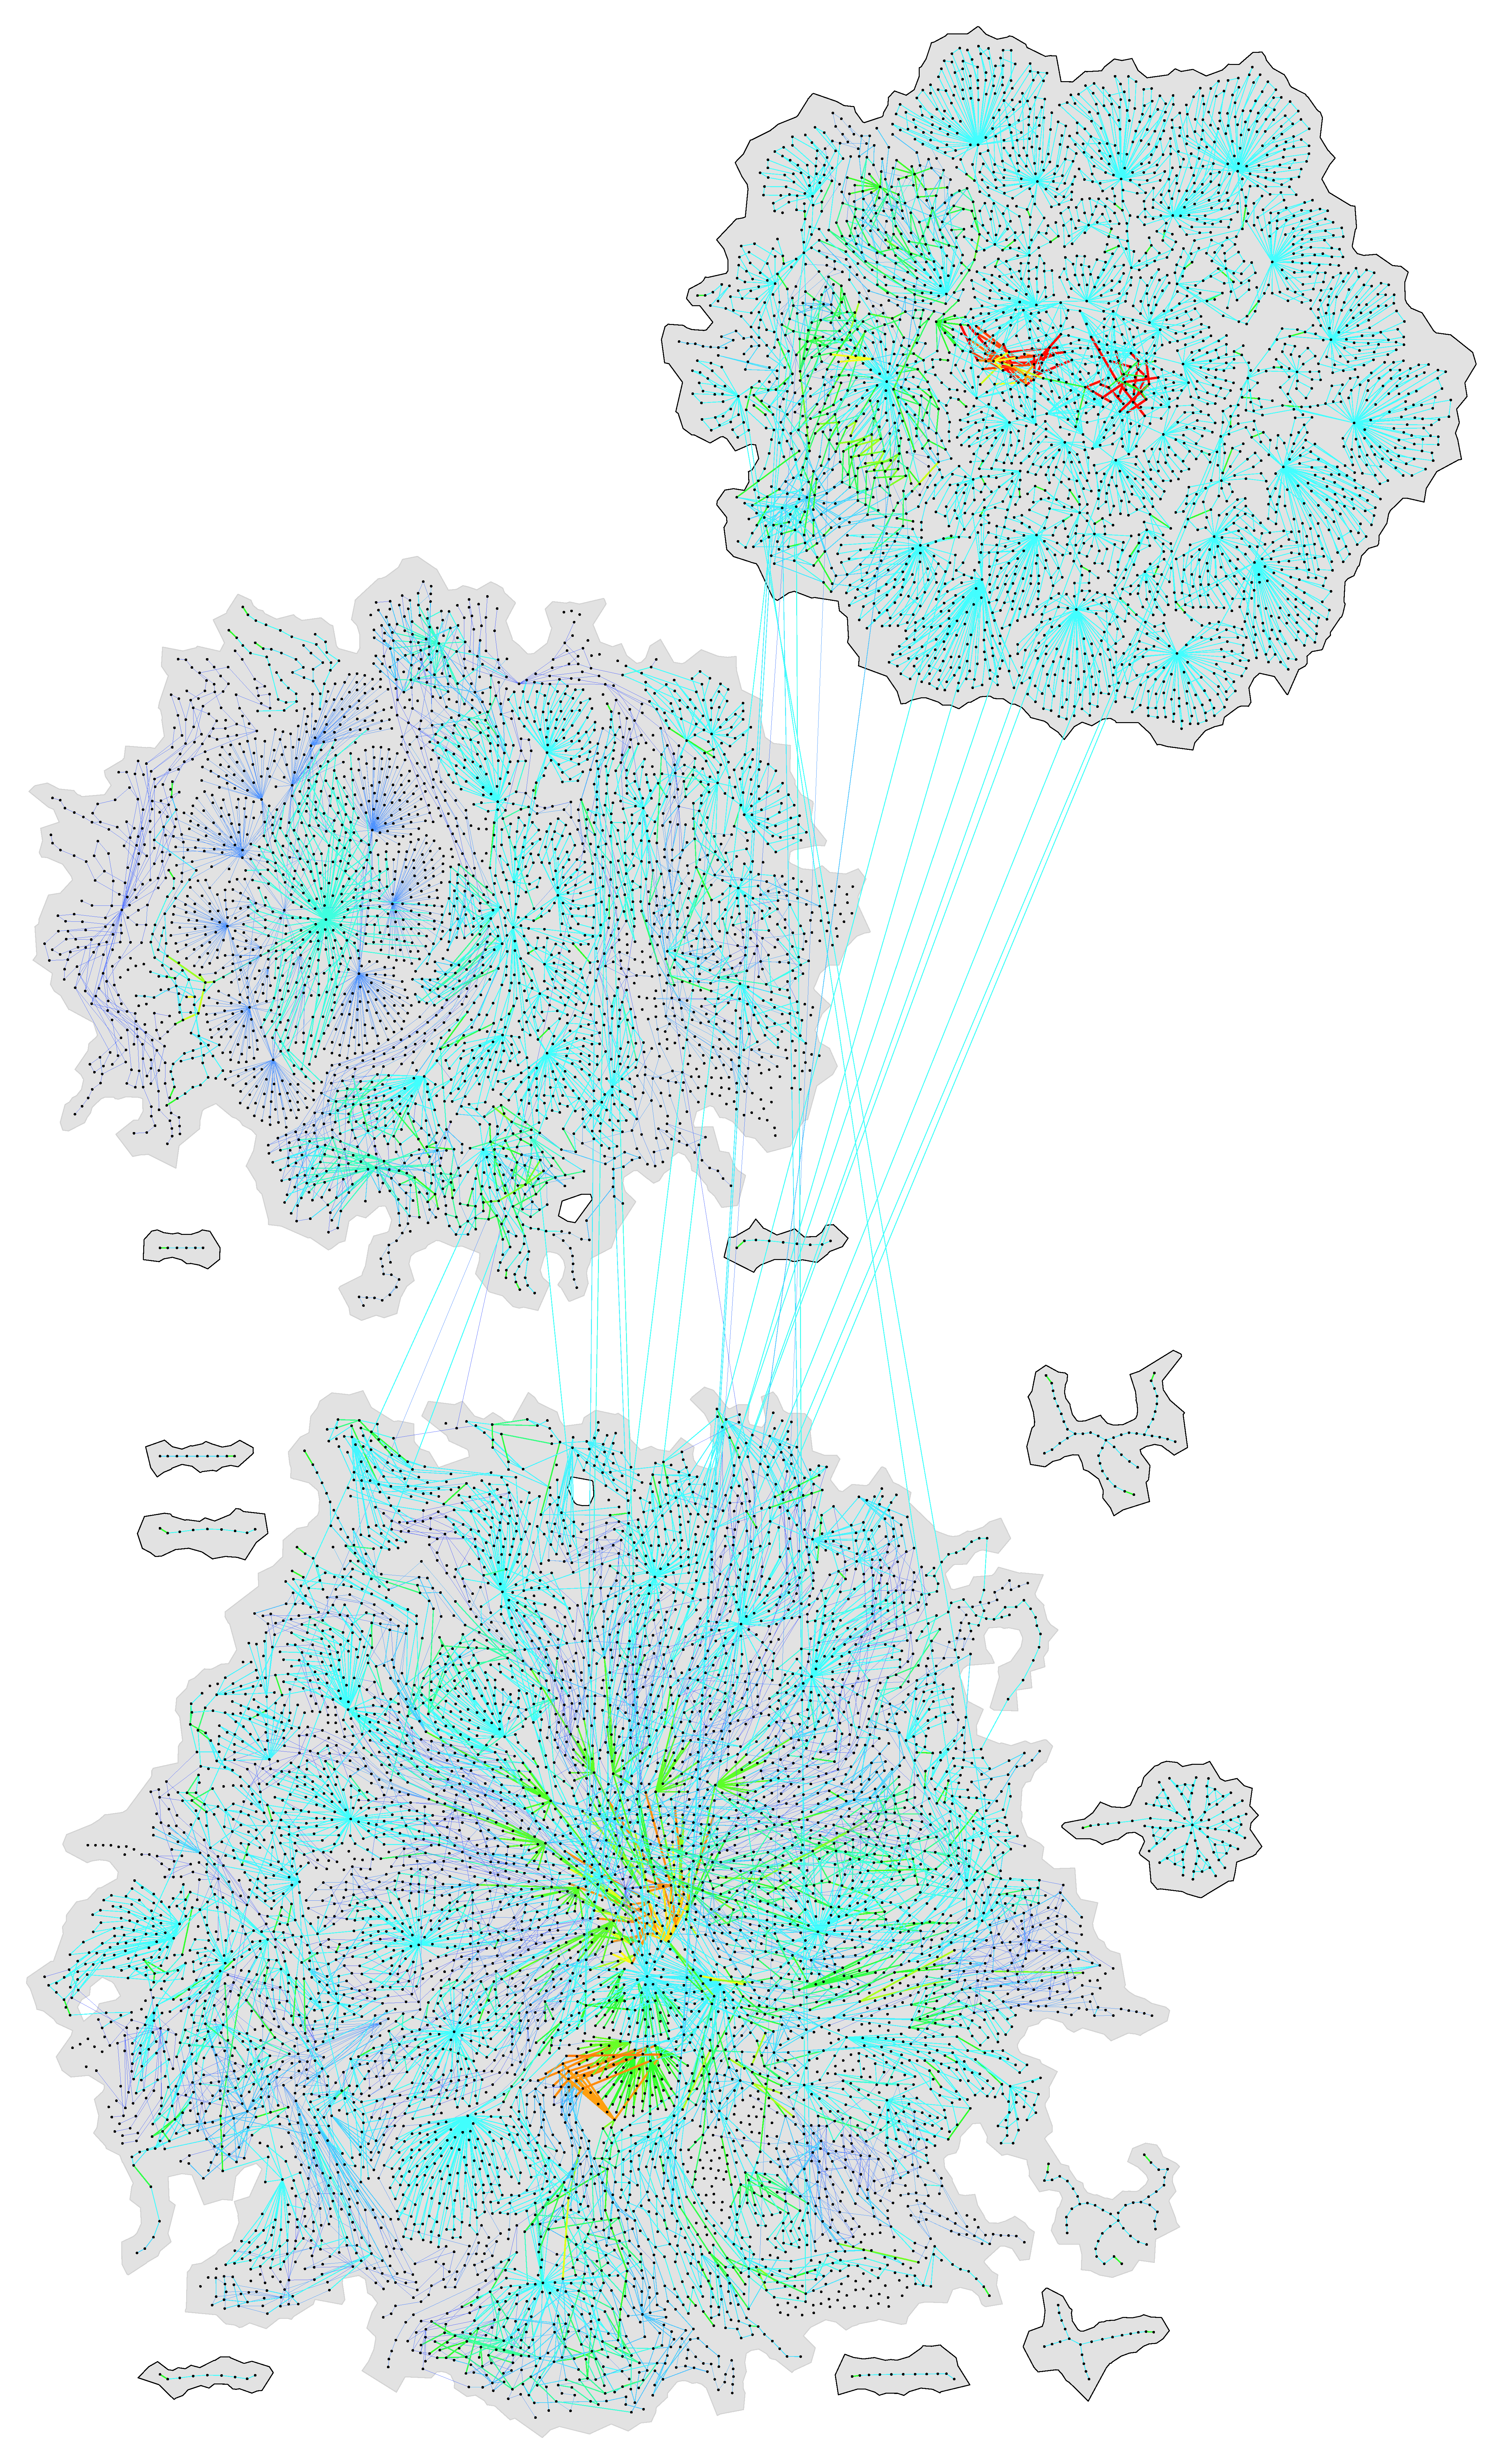
\includegraphics[clip=true,width=0.5\textwidth]{figs/s38584_2part.pdf}
\caption{Heatmap of messages sent during the ISCAS'89 s38584 simulation, partitioned into two partitions using the profile guided algorithm.}
\end{figure}

\begin{figure}
\centering
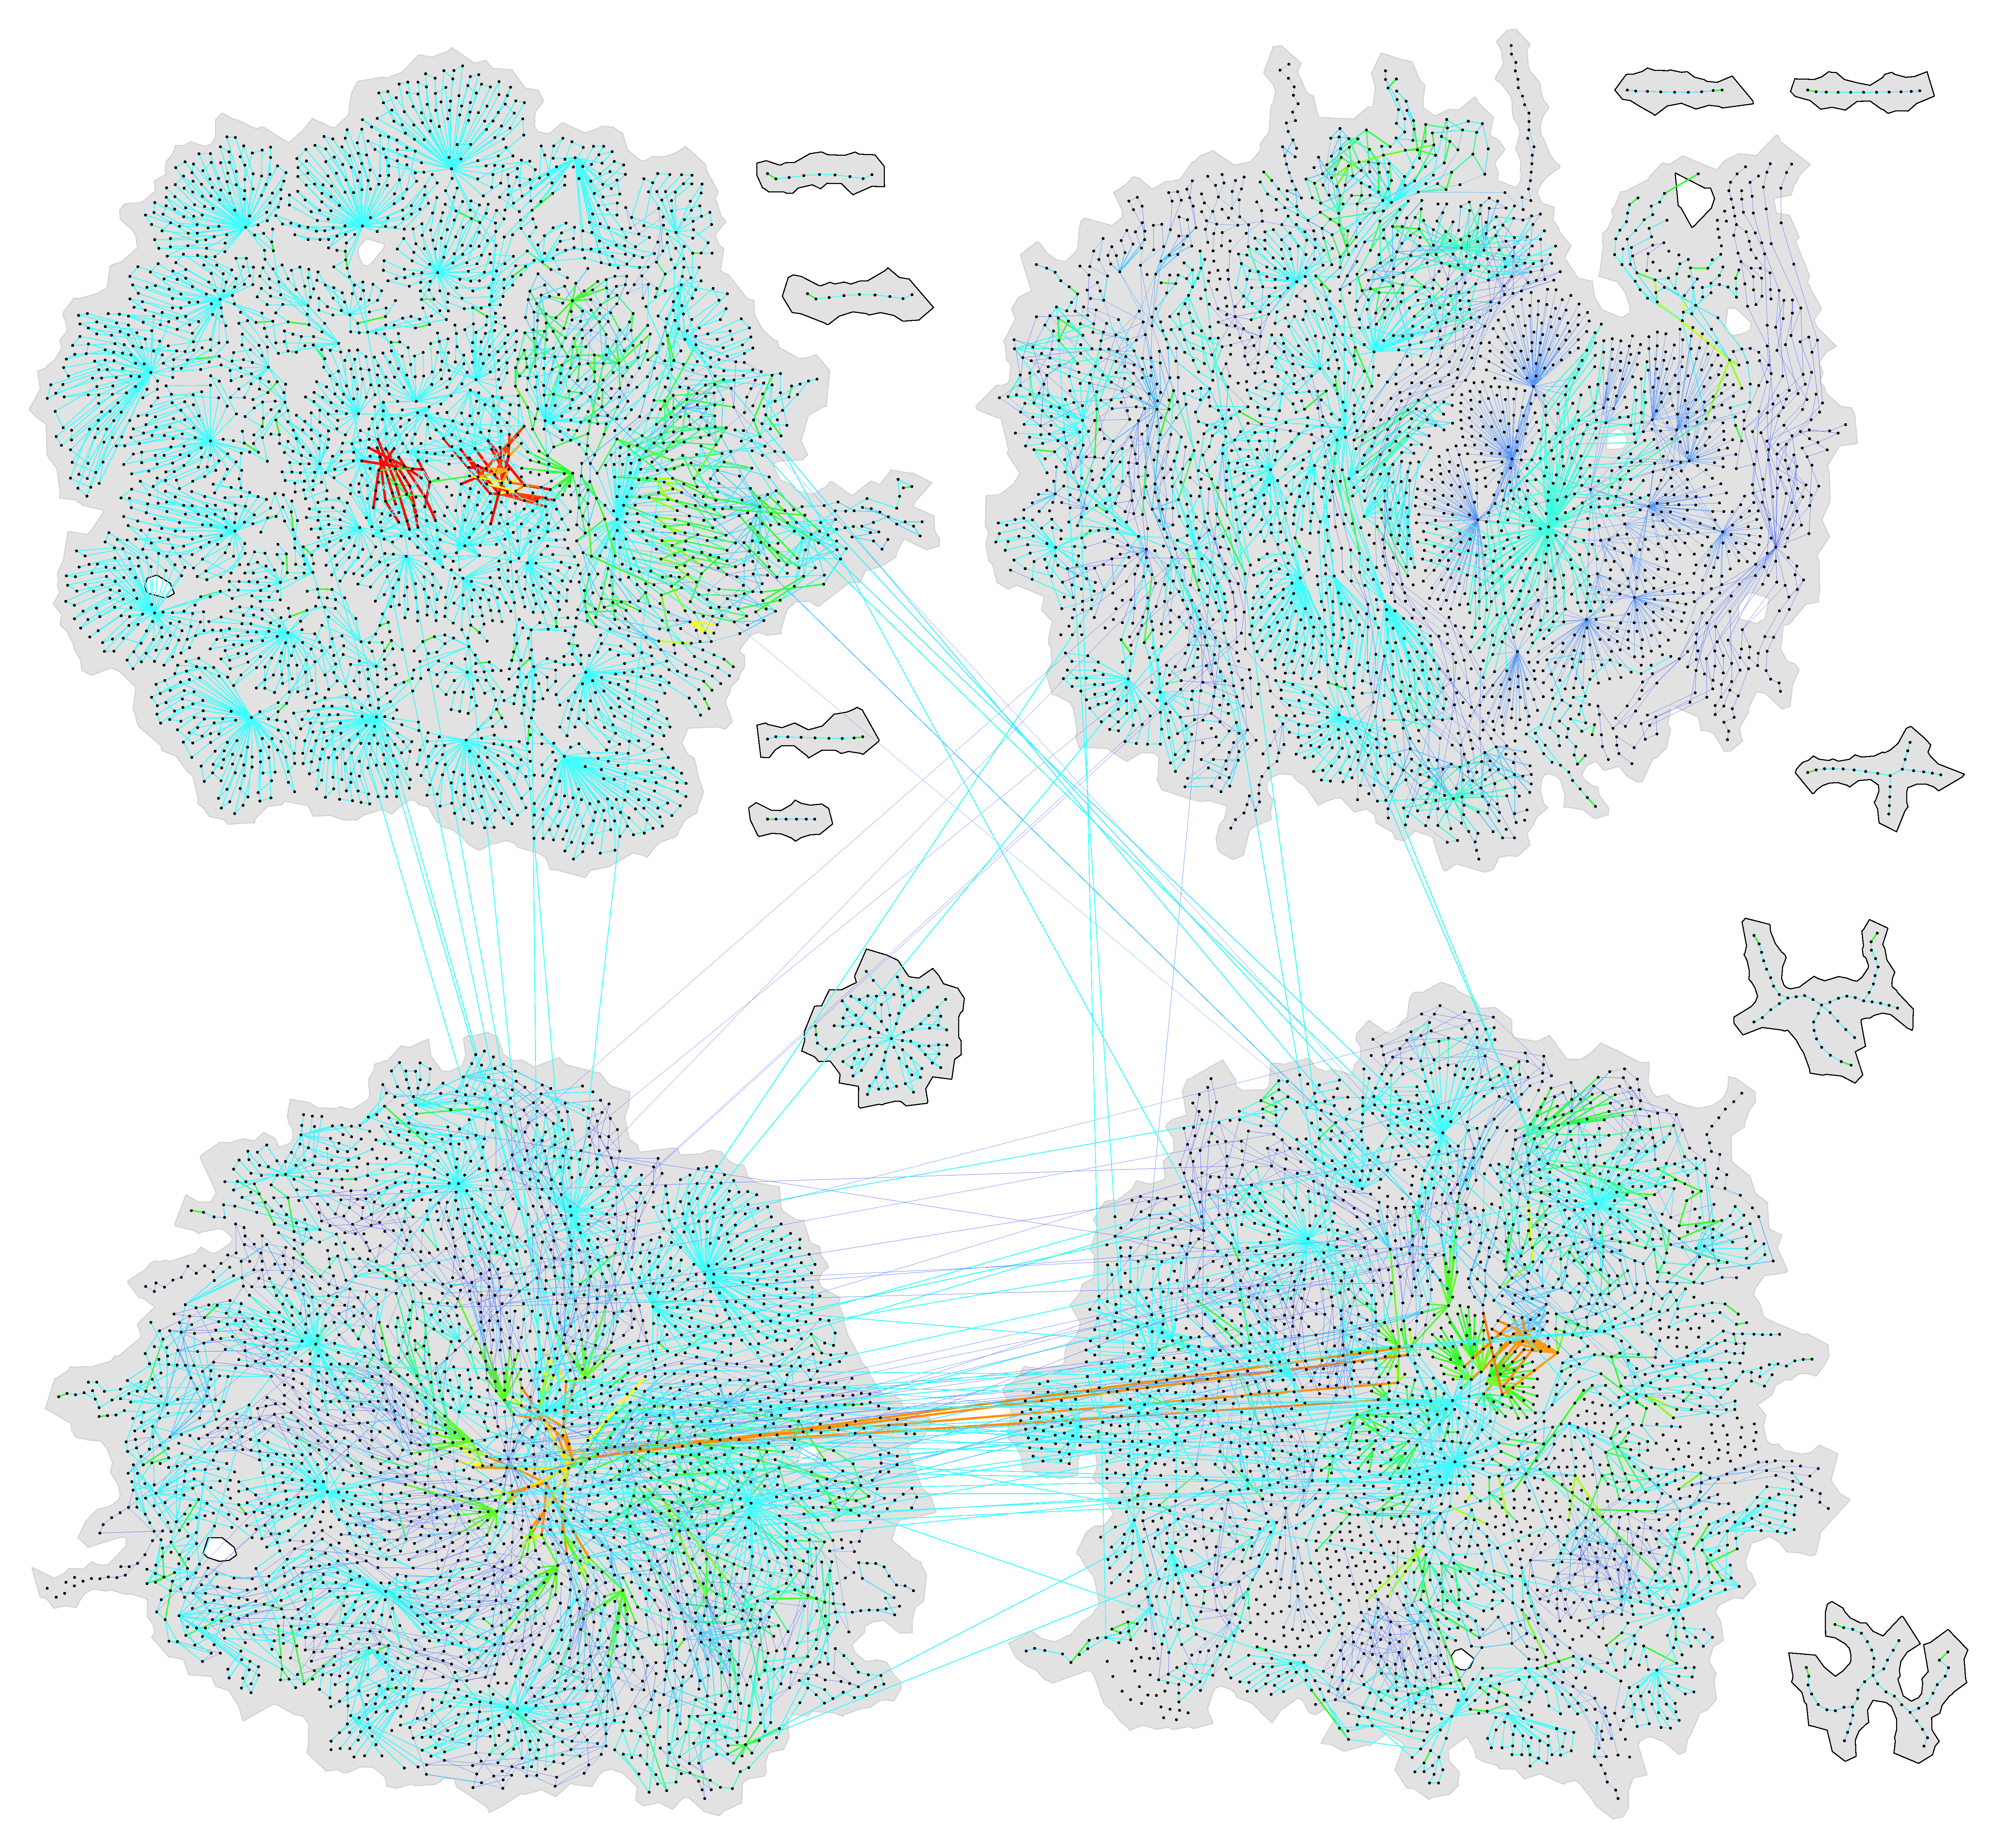
\includegraphics[clip=true,width=0.5\textwidth]{figs/s38584_4part.pdf}
\caption{Heatmap of messages sent during the ISCAS'89 s38584 simulation, partitioned into four partitions using the profile guided algorithm.}
\end{figure}

\begin{figure}
\centering
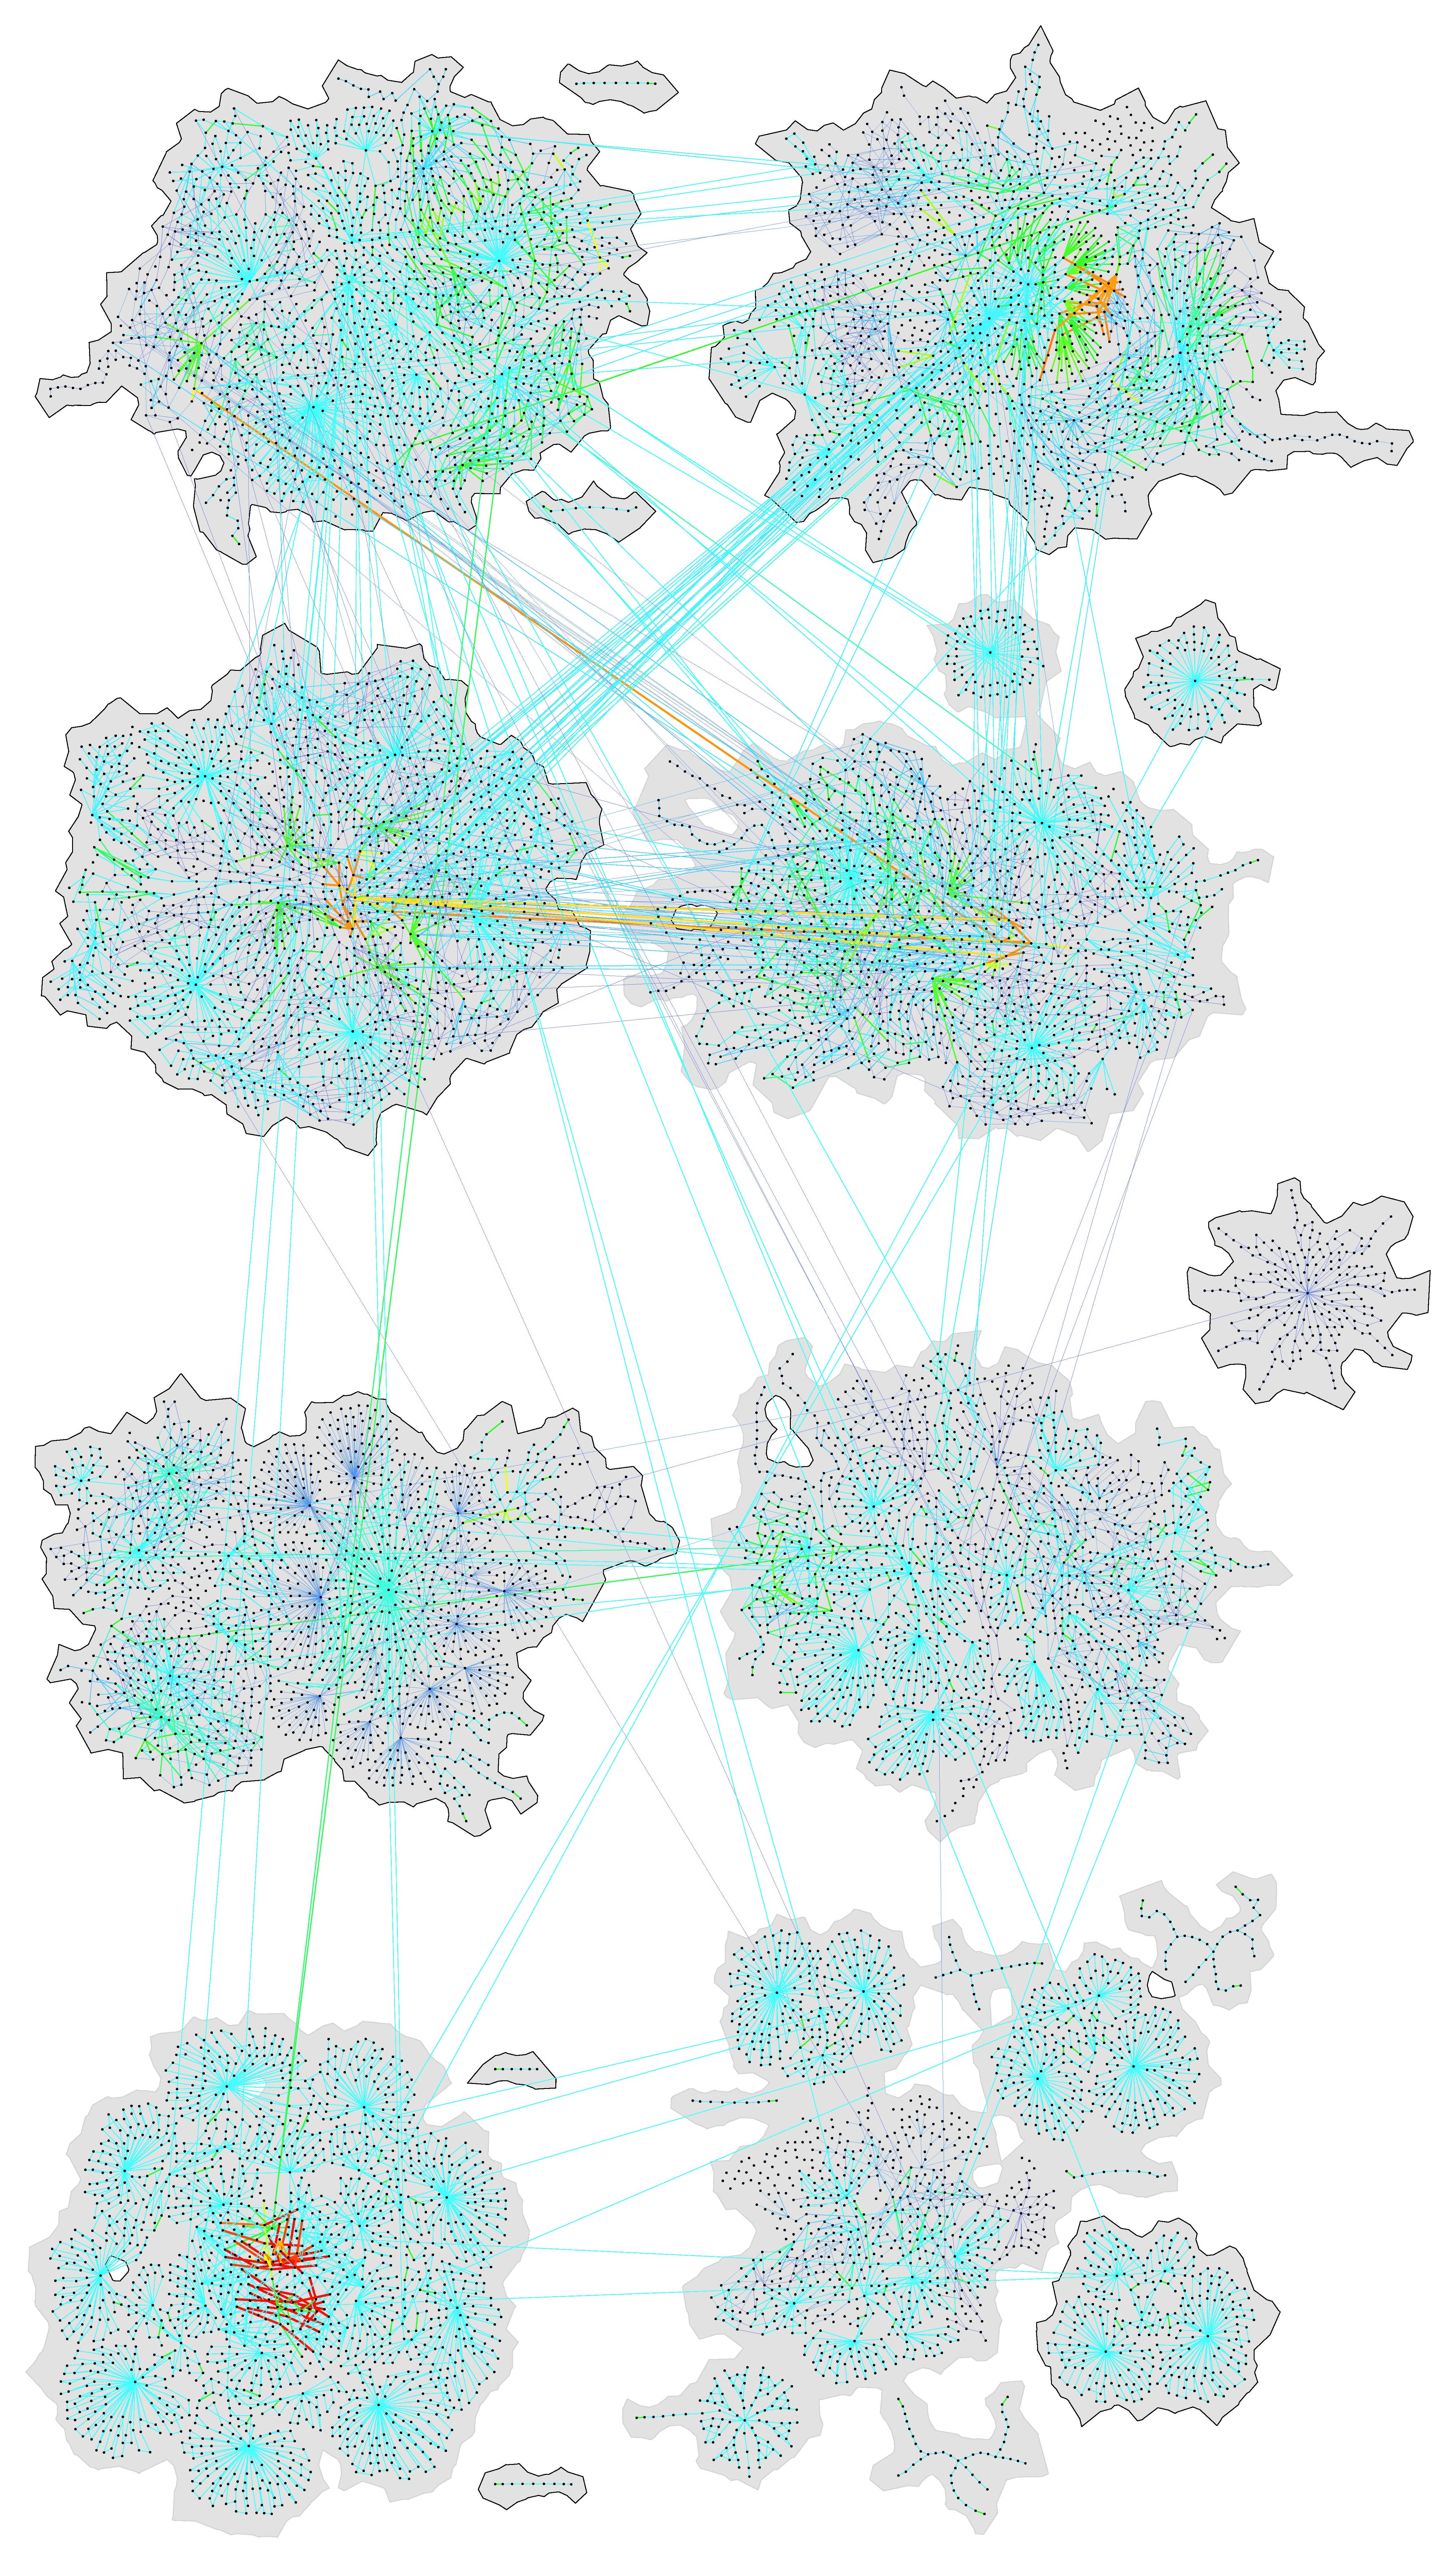
\includegraphics[clip=true,width=0.5\textwidth]{figs/s38584_8part.pdf}
\caption{Heatmap of messages sent during the ISCAS'89 s38584 simulation, partitioned into eight partitions using the profile guided algorithm.}
\end{figure}

\begin{figure}
\centering
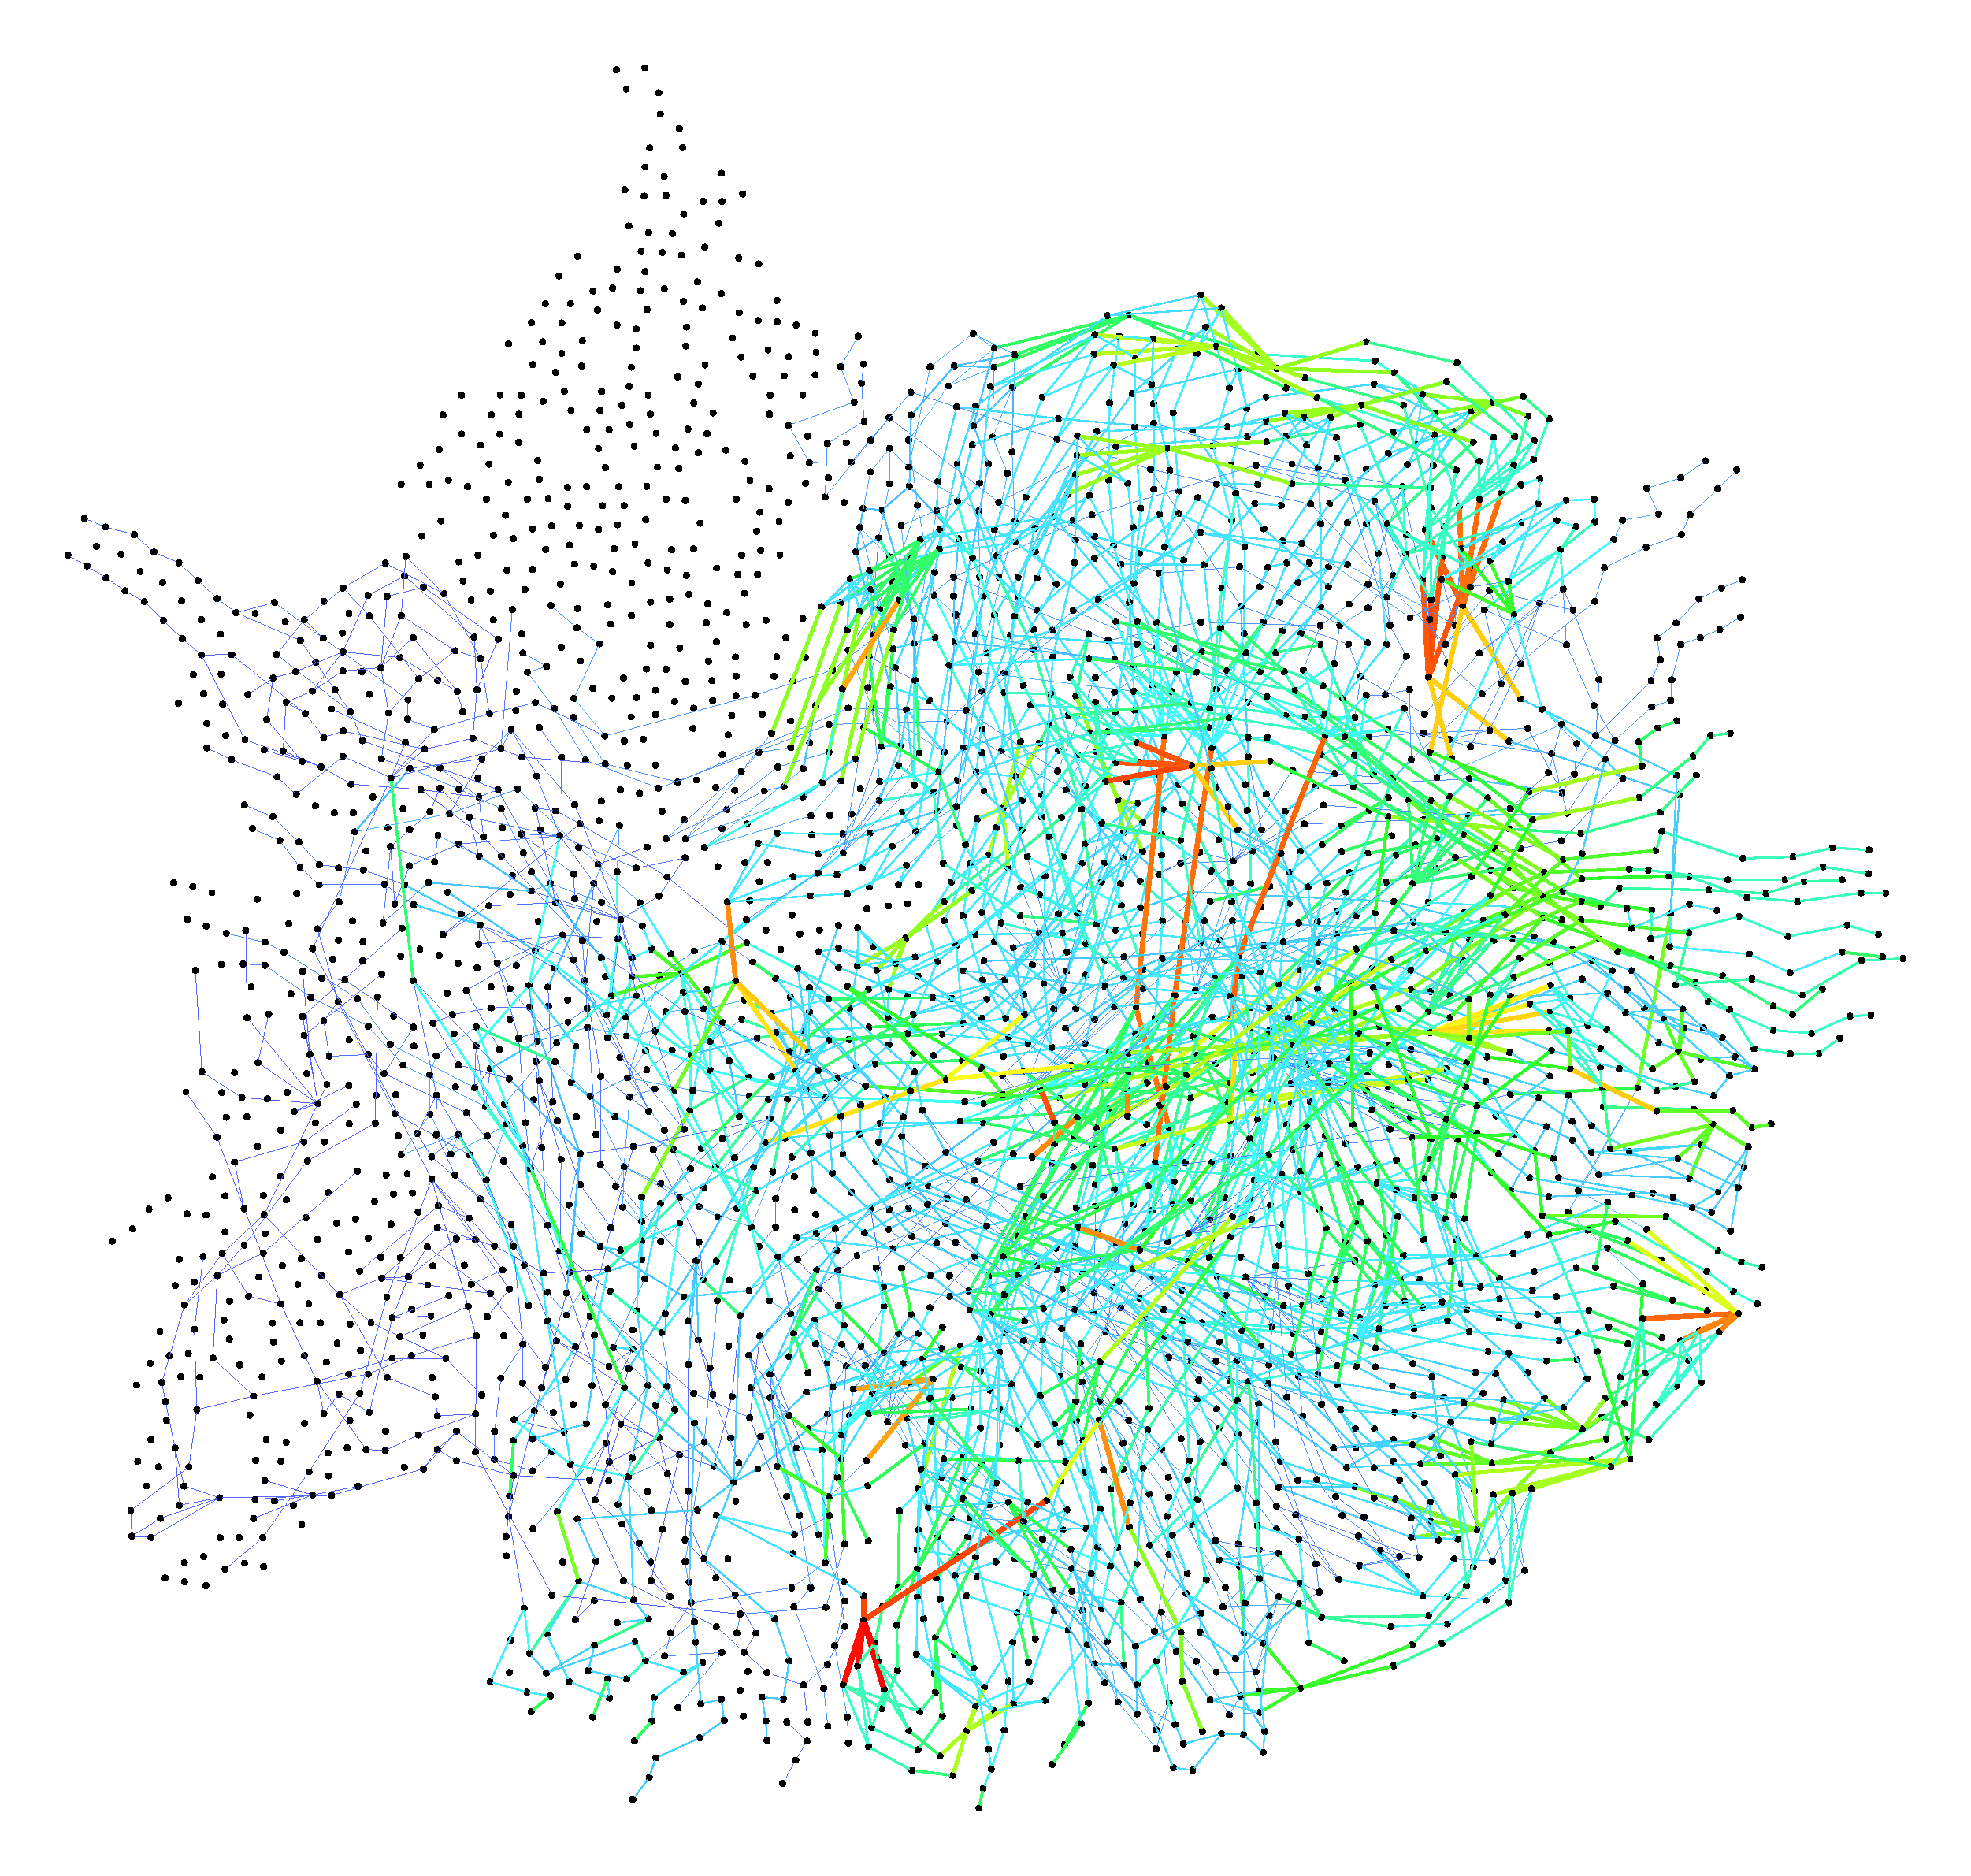
\includegraphics[clip=true,width=0.5\textwidth]{figs/s5378.pdf}
\caption{Heatmap of messages sent during the ISCAS'89 s5378 simulation.}
\end{figure}

\begin{figure}
\centering
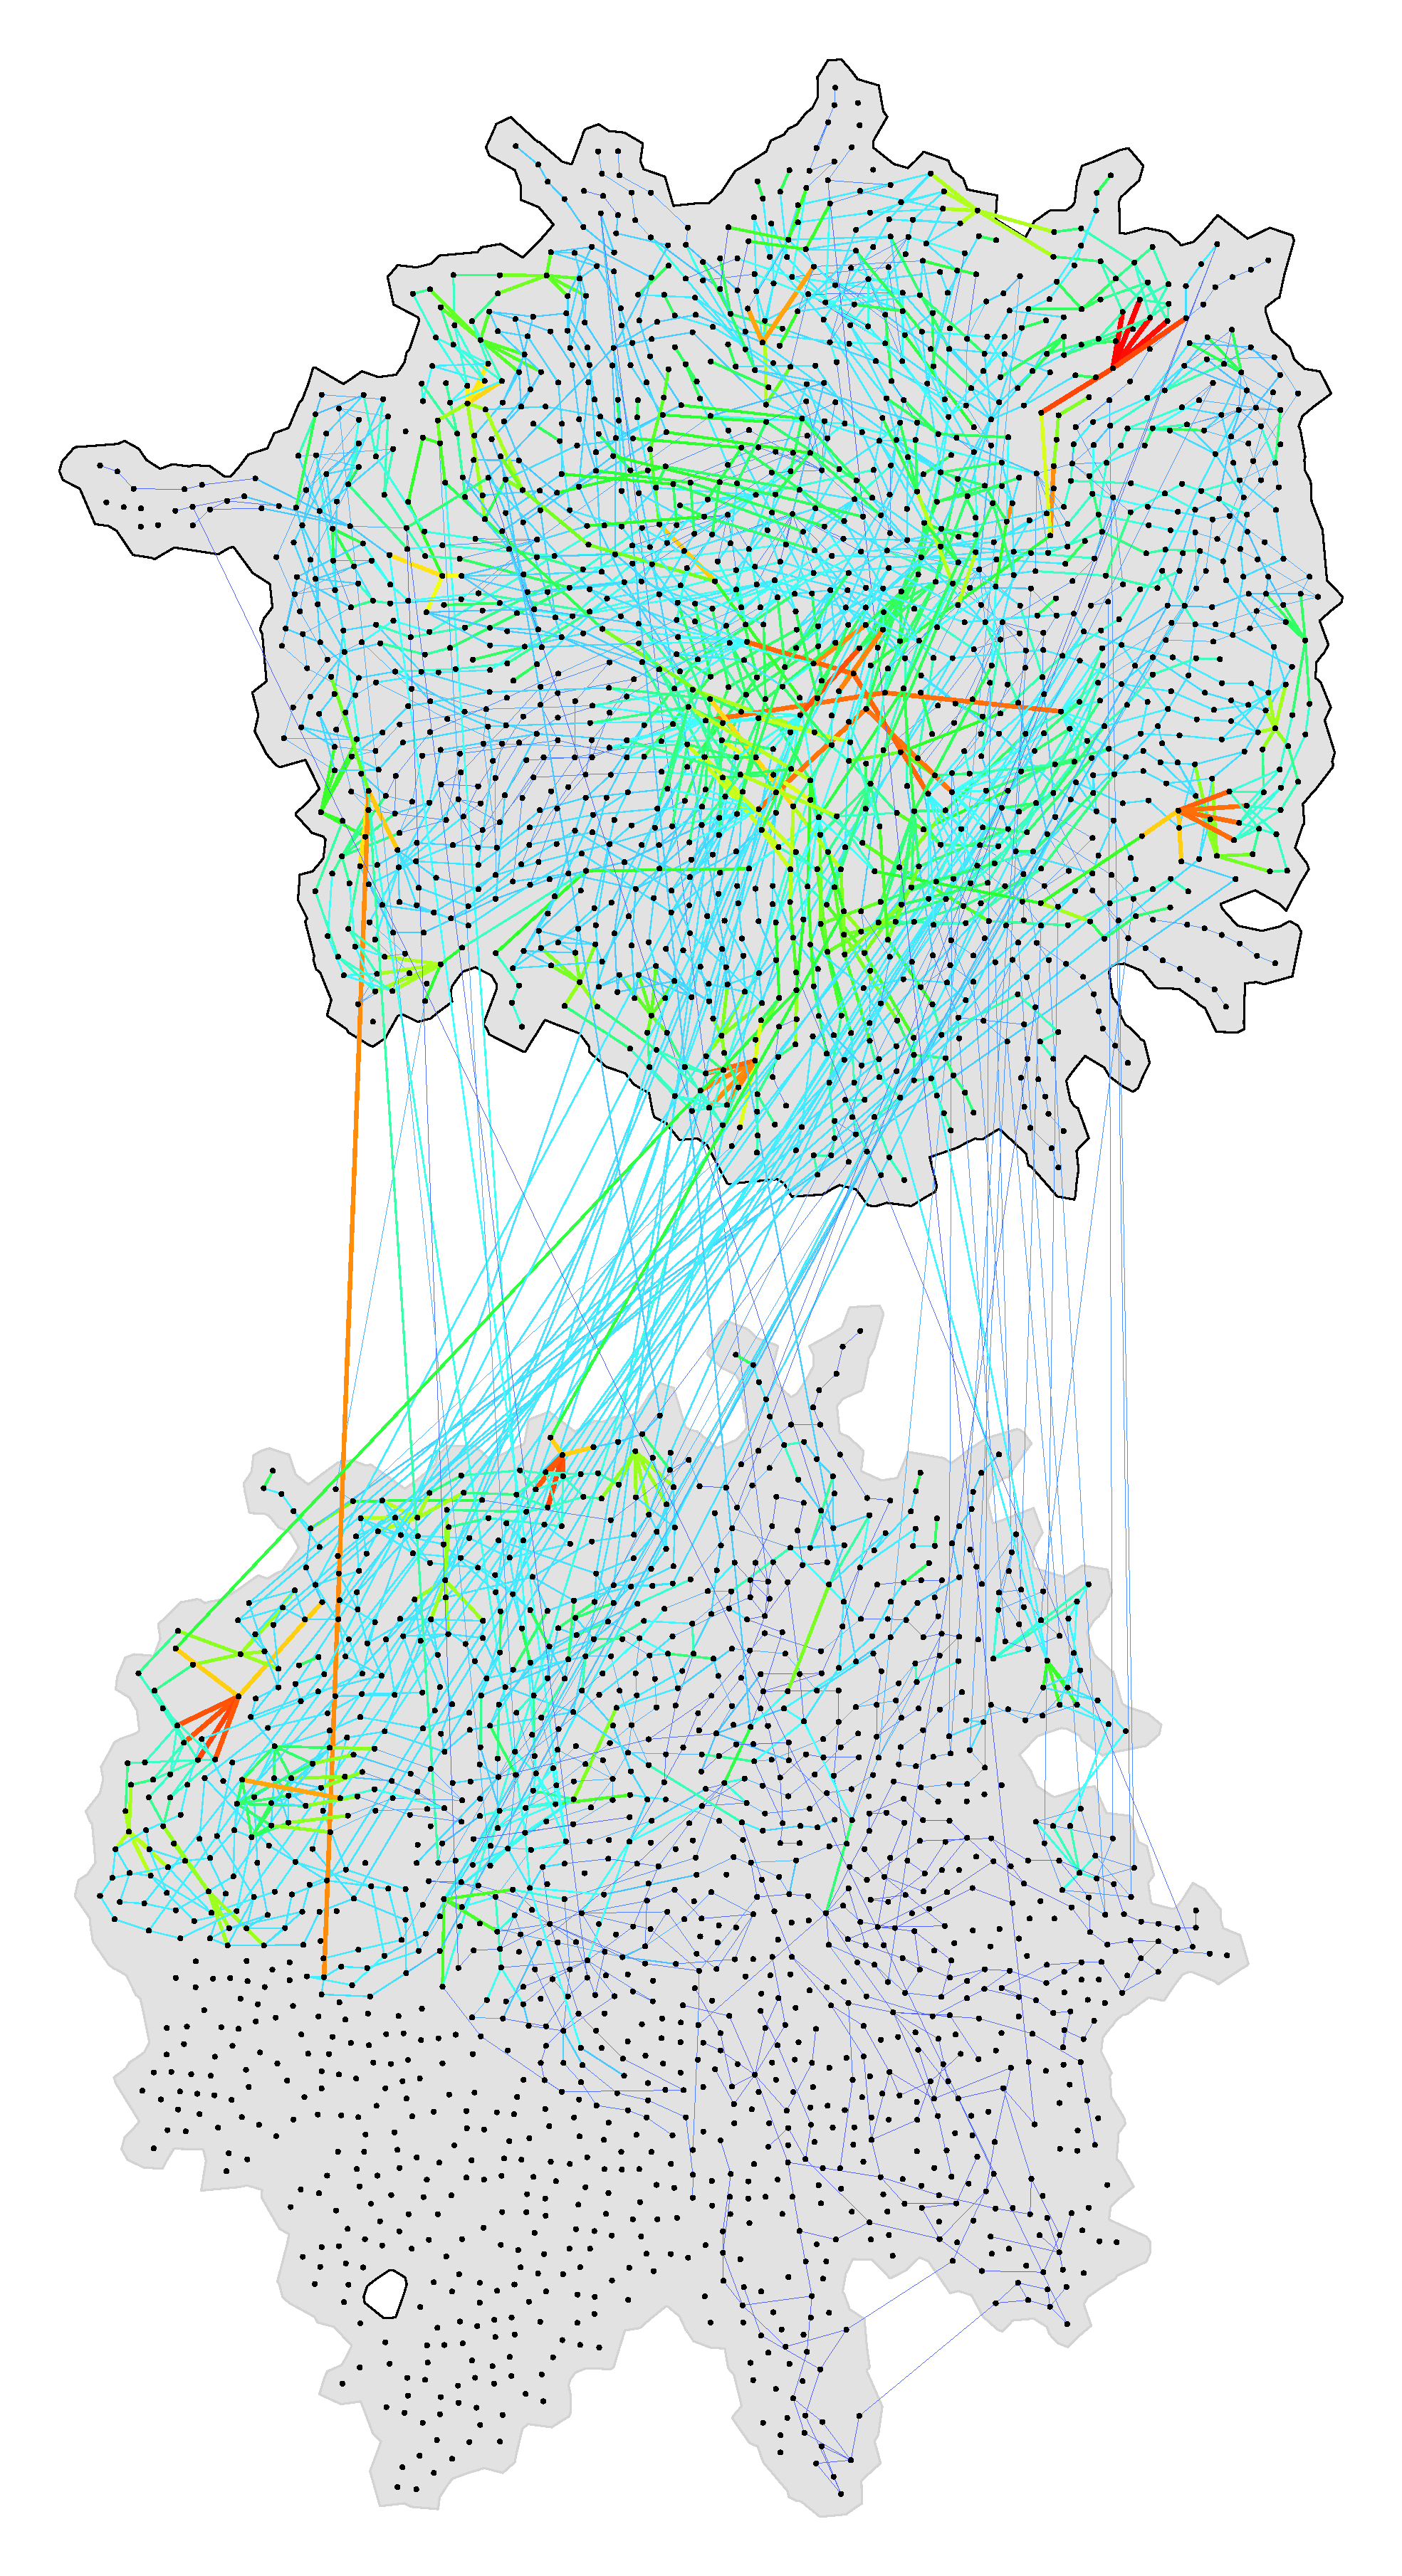
\includegraphics[clip=true,width=0.5\textwidth]{figs/s5378_2part.pdf}
\caption{Heatmap of messages sent during the ISCAS'89 s5378 simulation, partitioned into two partitions using the profile guided algorithm.}
\end{figure}

\begin{figure}
\centering
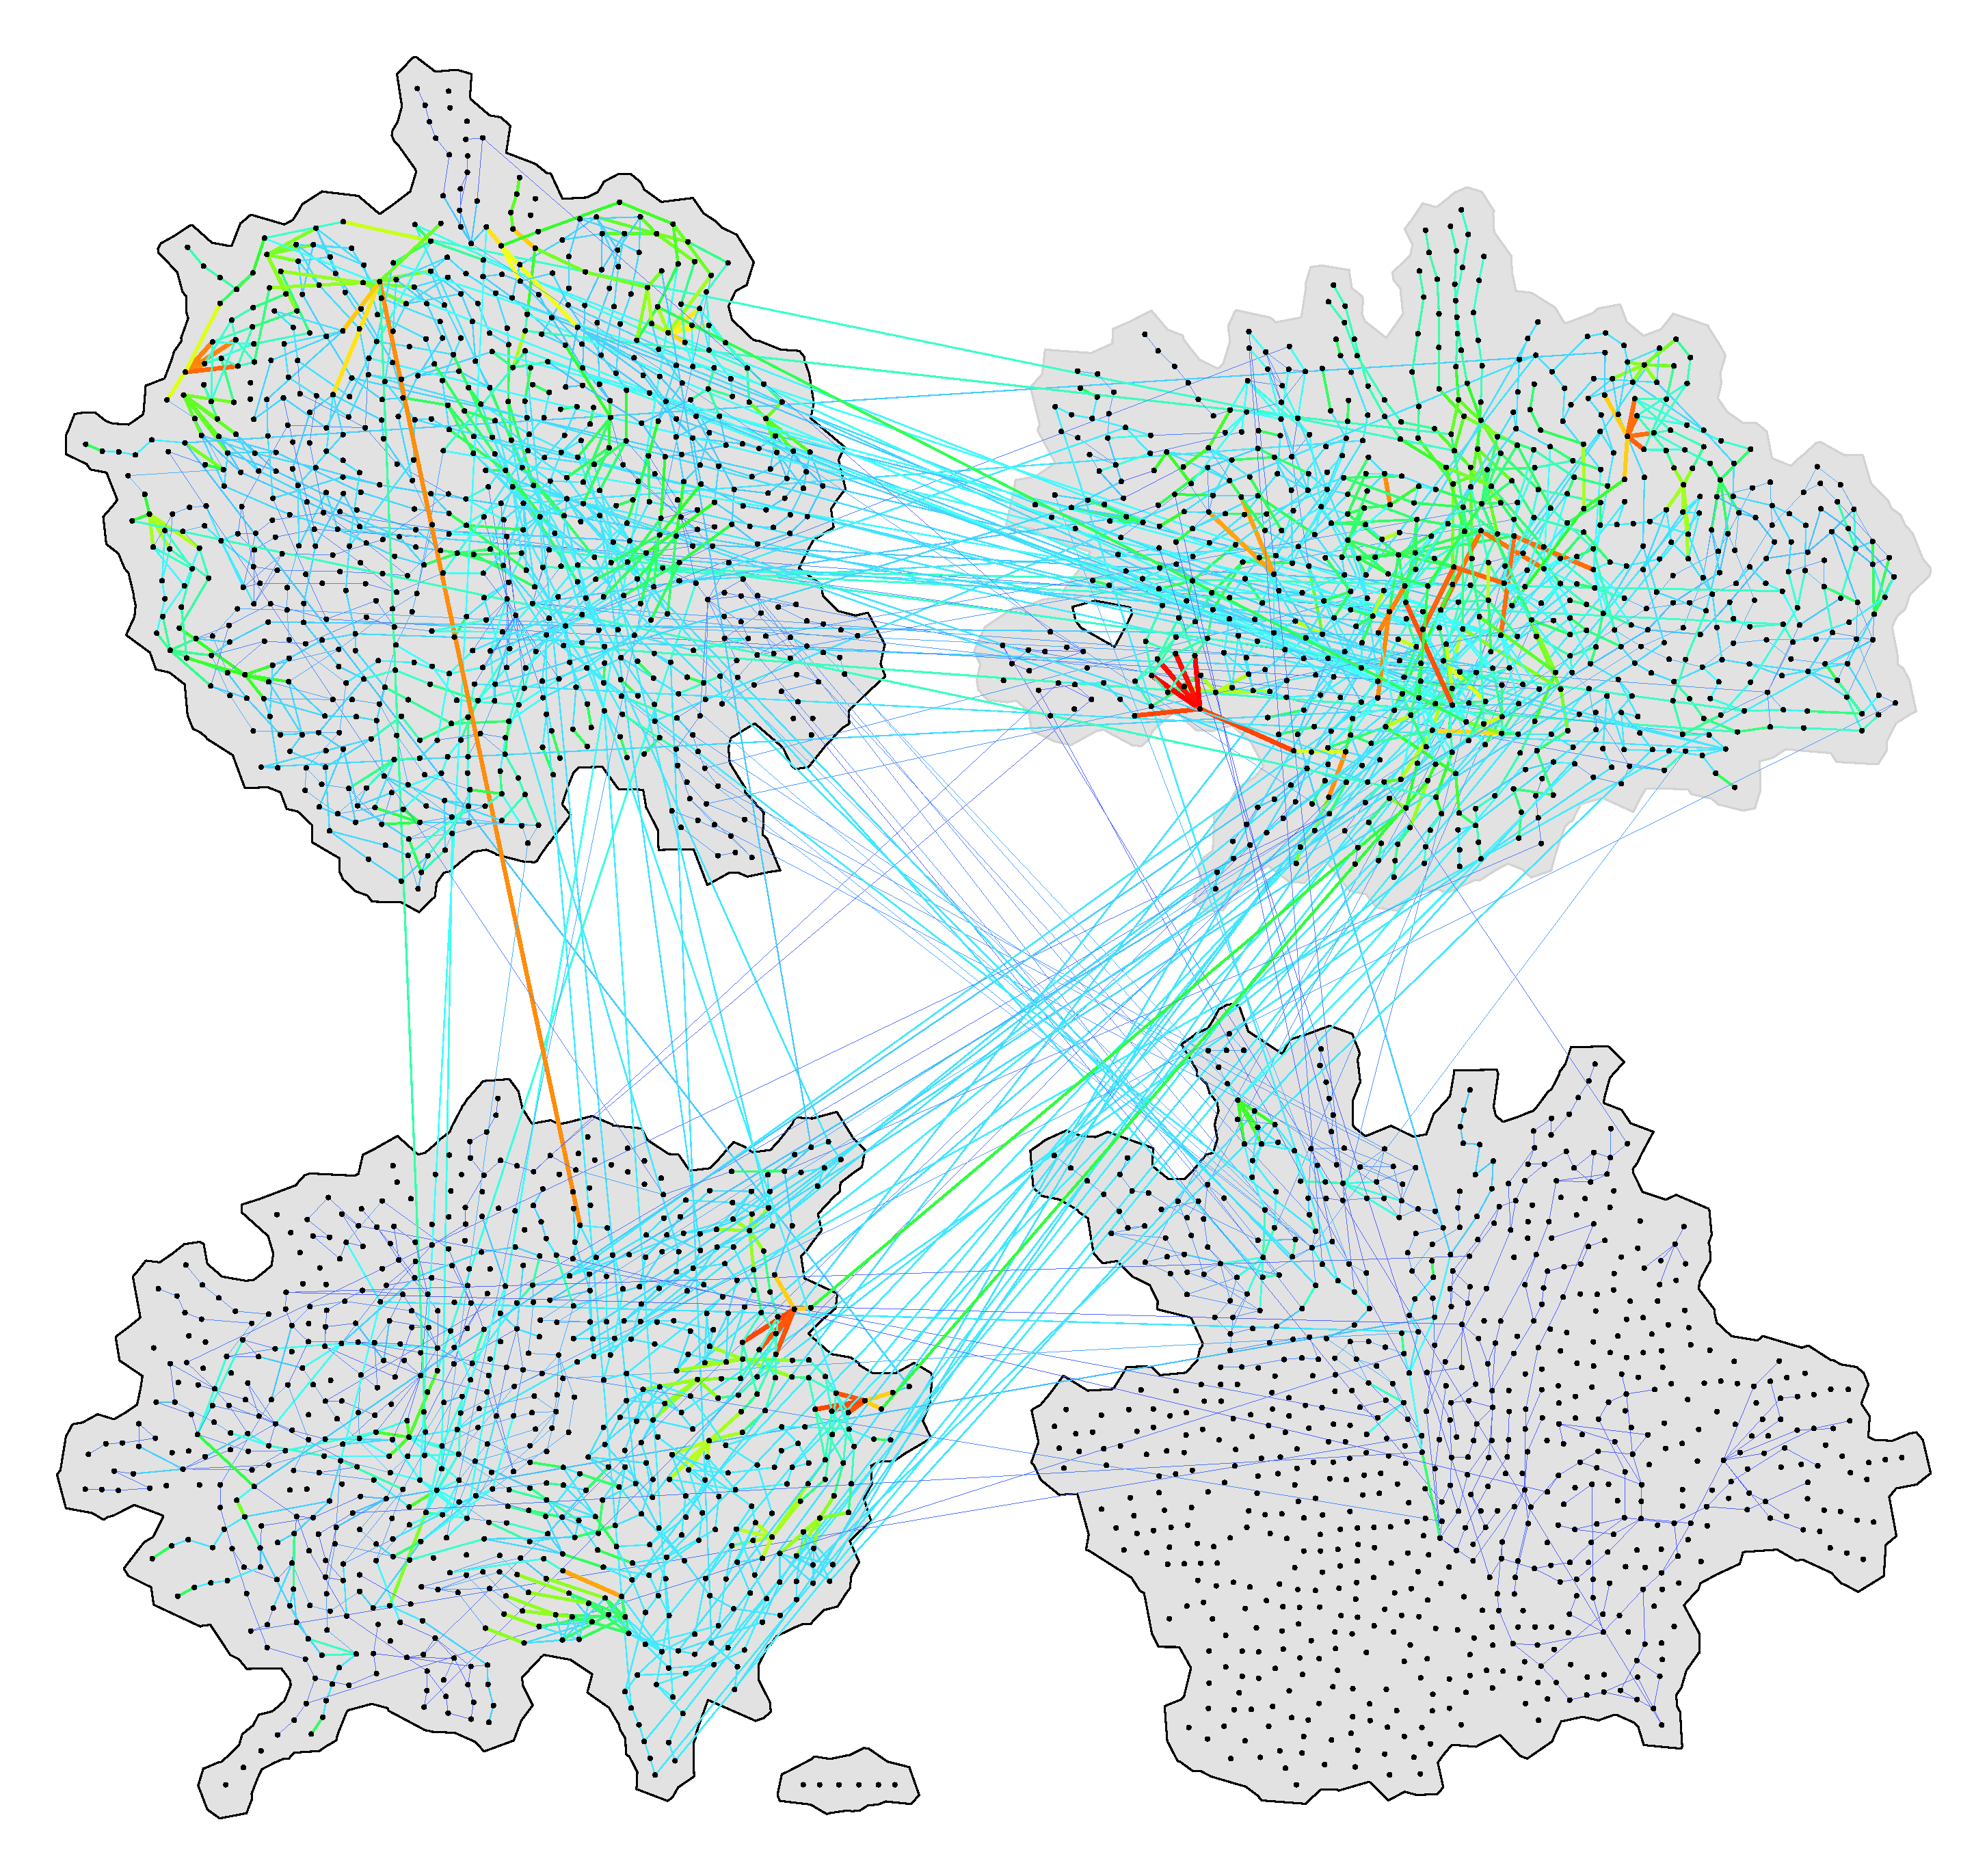
\includegraphics[clip=true,width=0.5\textwidth]{figs/s5378_4part.pdf}
\caption{Heatmap of messages sent during the ISCAS'89 s5378 simulation, partitioned into four partitions using the profile guided algorithm.}
\end{figure}

\begin{figure}
\centering
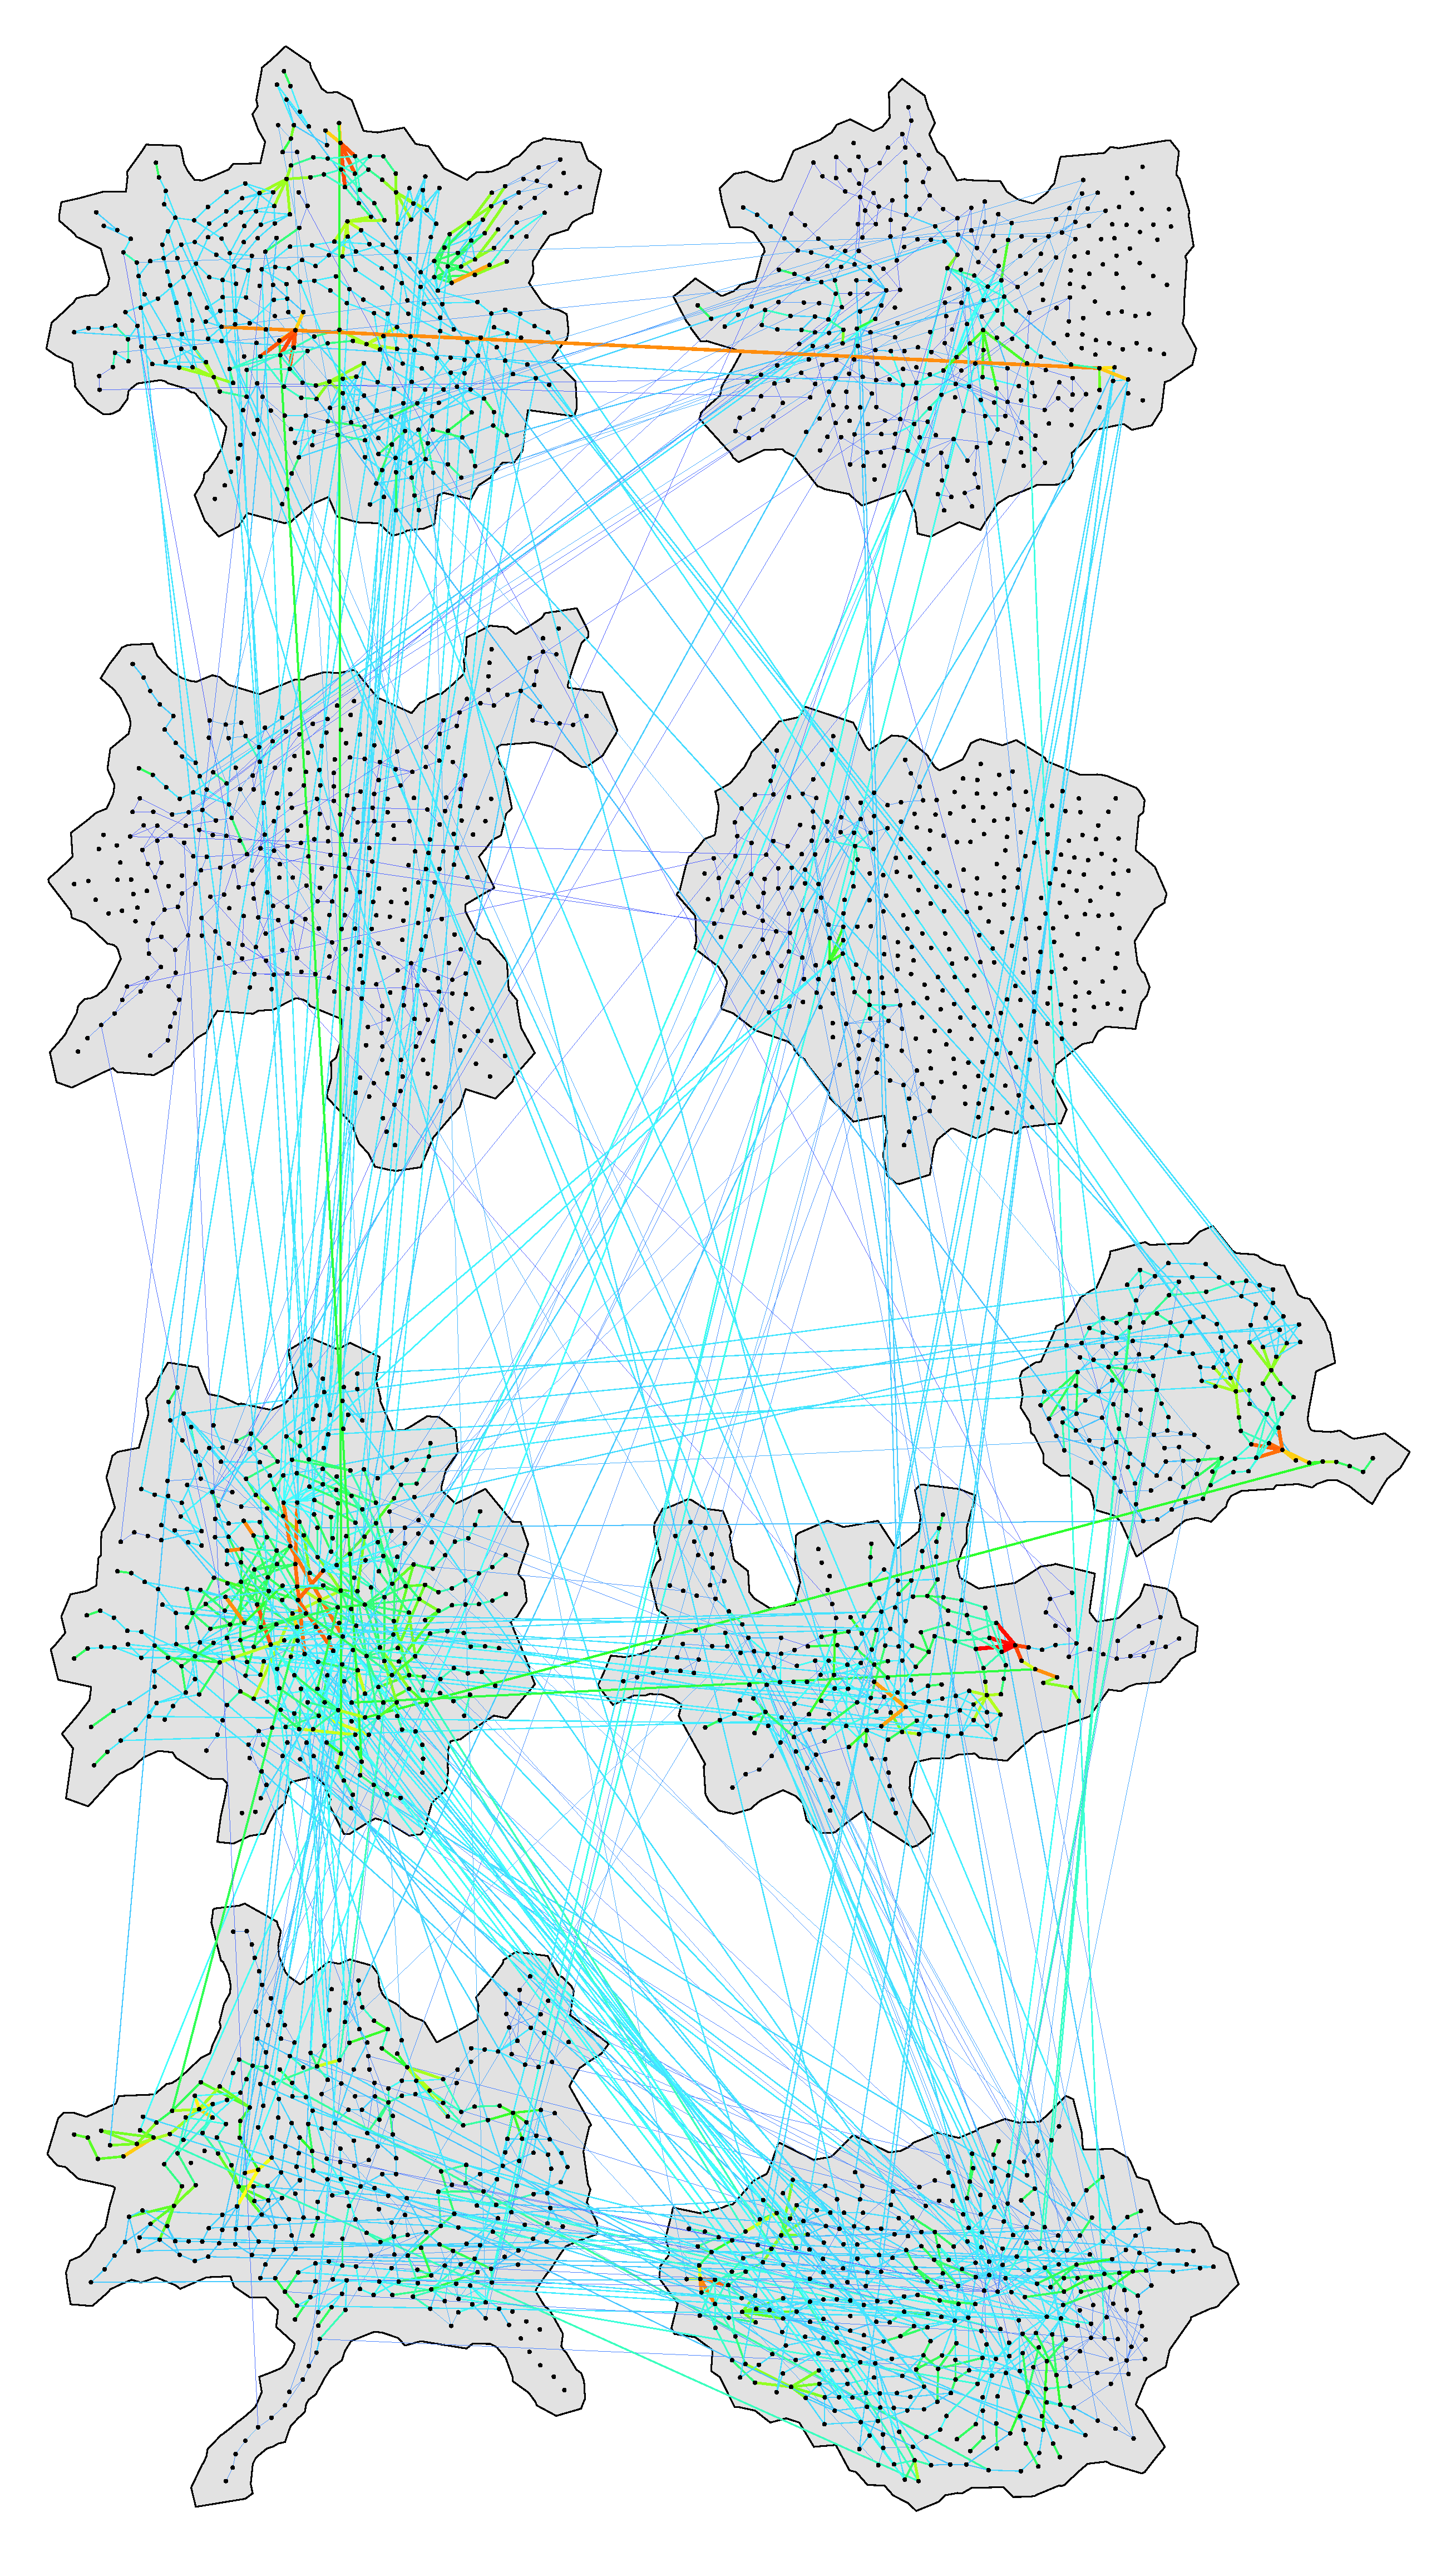
\includegraphics[clip=true,width=0.5\textwidth]{figs/s5378_8part.pdf}
\caption{Heatmap of messages sent during the ISCAS'89 s5378 simulation, partitioned into eight partitions using the profile guided algorithm.}
\end{figure}

\begin{figure}
\centering
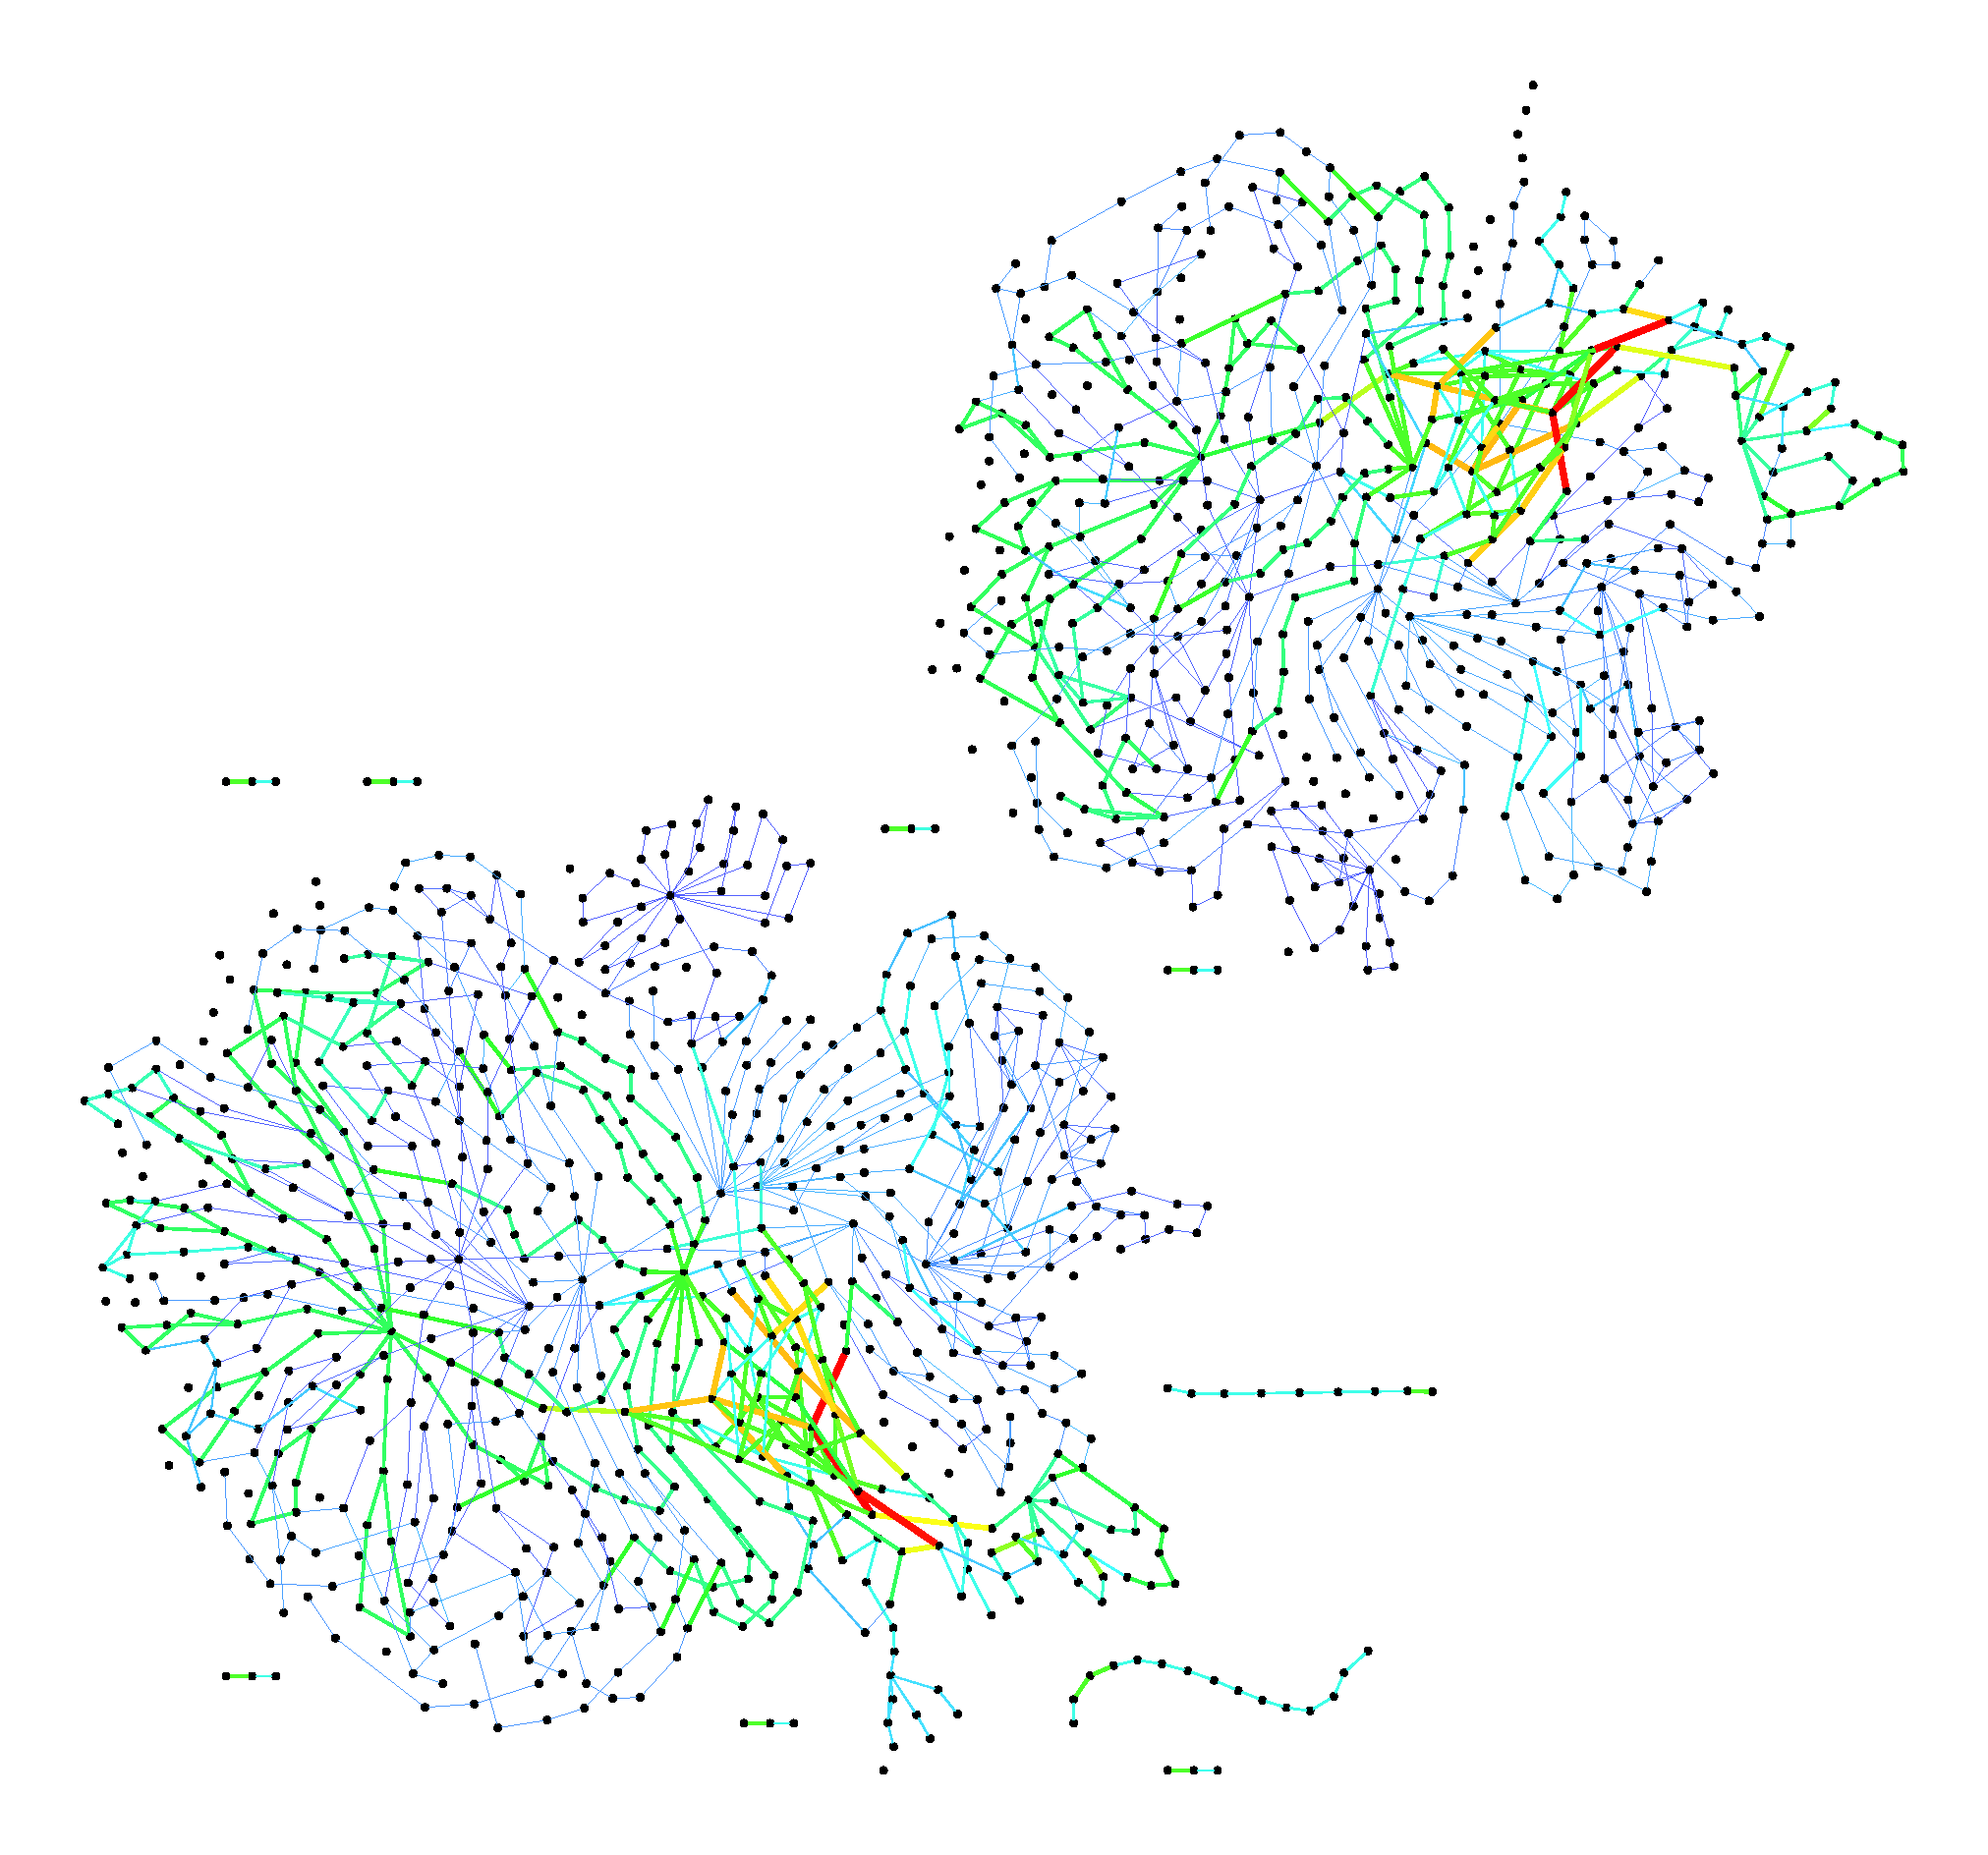
\includegraphics[clip=true,width=0.5\textwidth]{figs/s9234.pdf}
\caption{Heatmap of messages sent during the ISCAS'89 s9234 simulation.}
\end{figure}

\begin{figure}
\centering
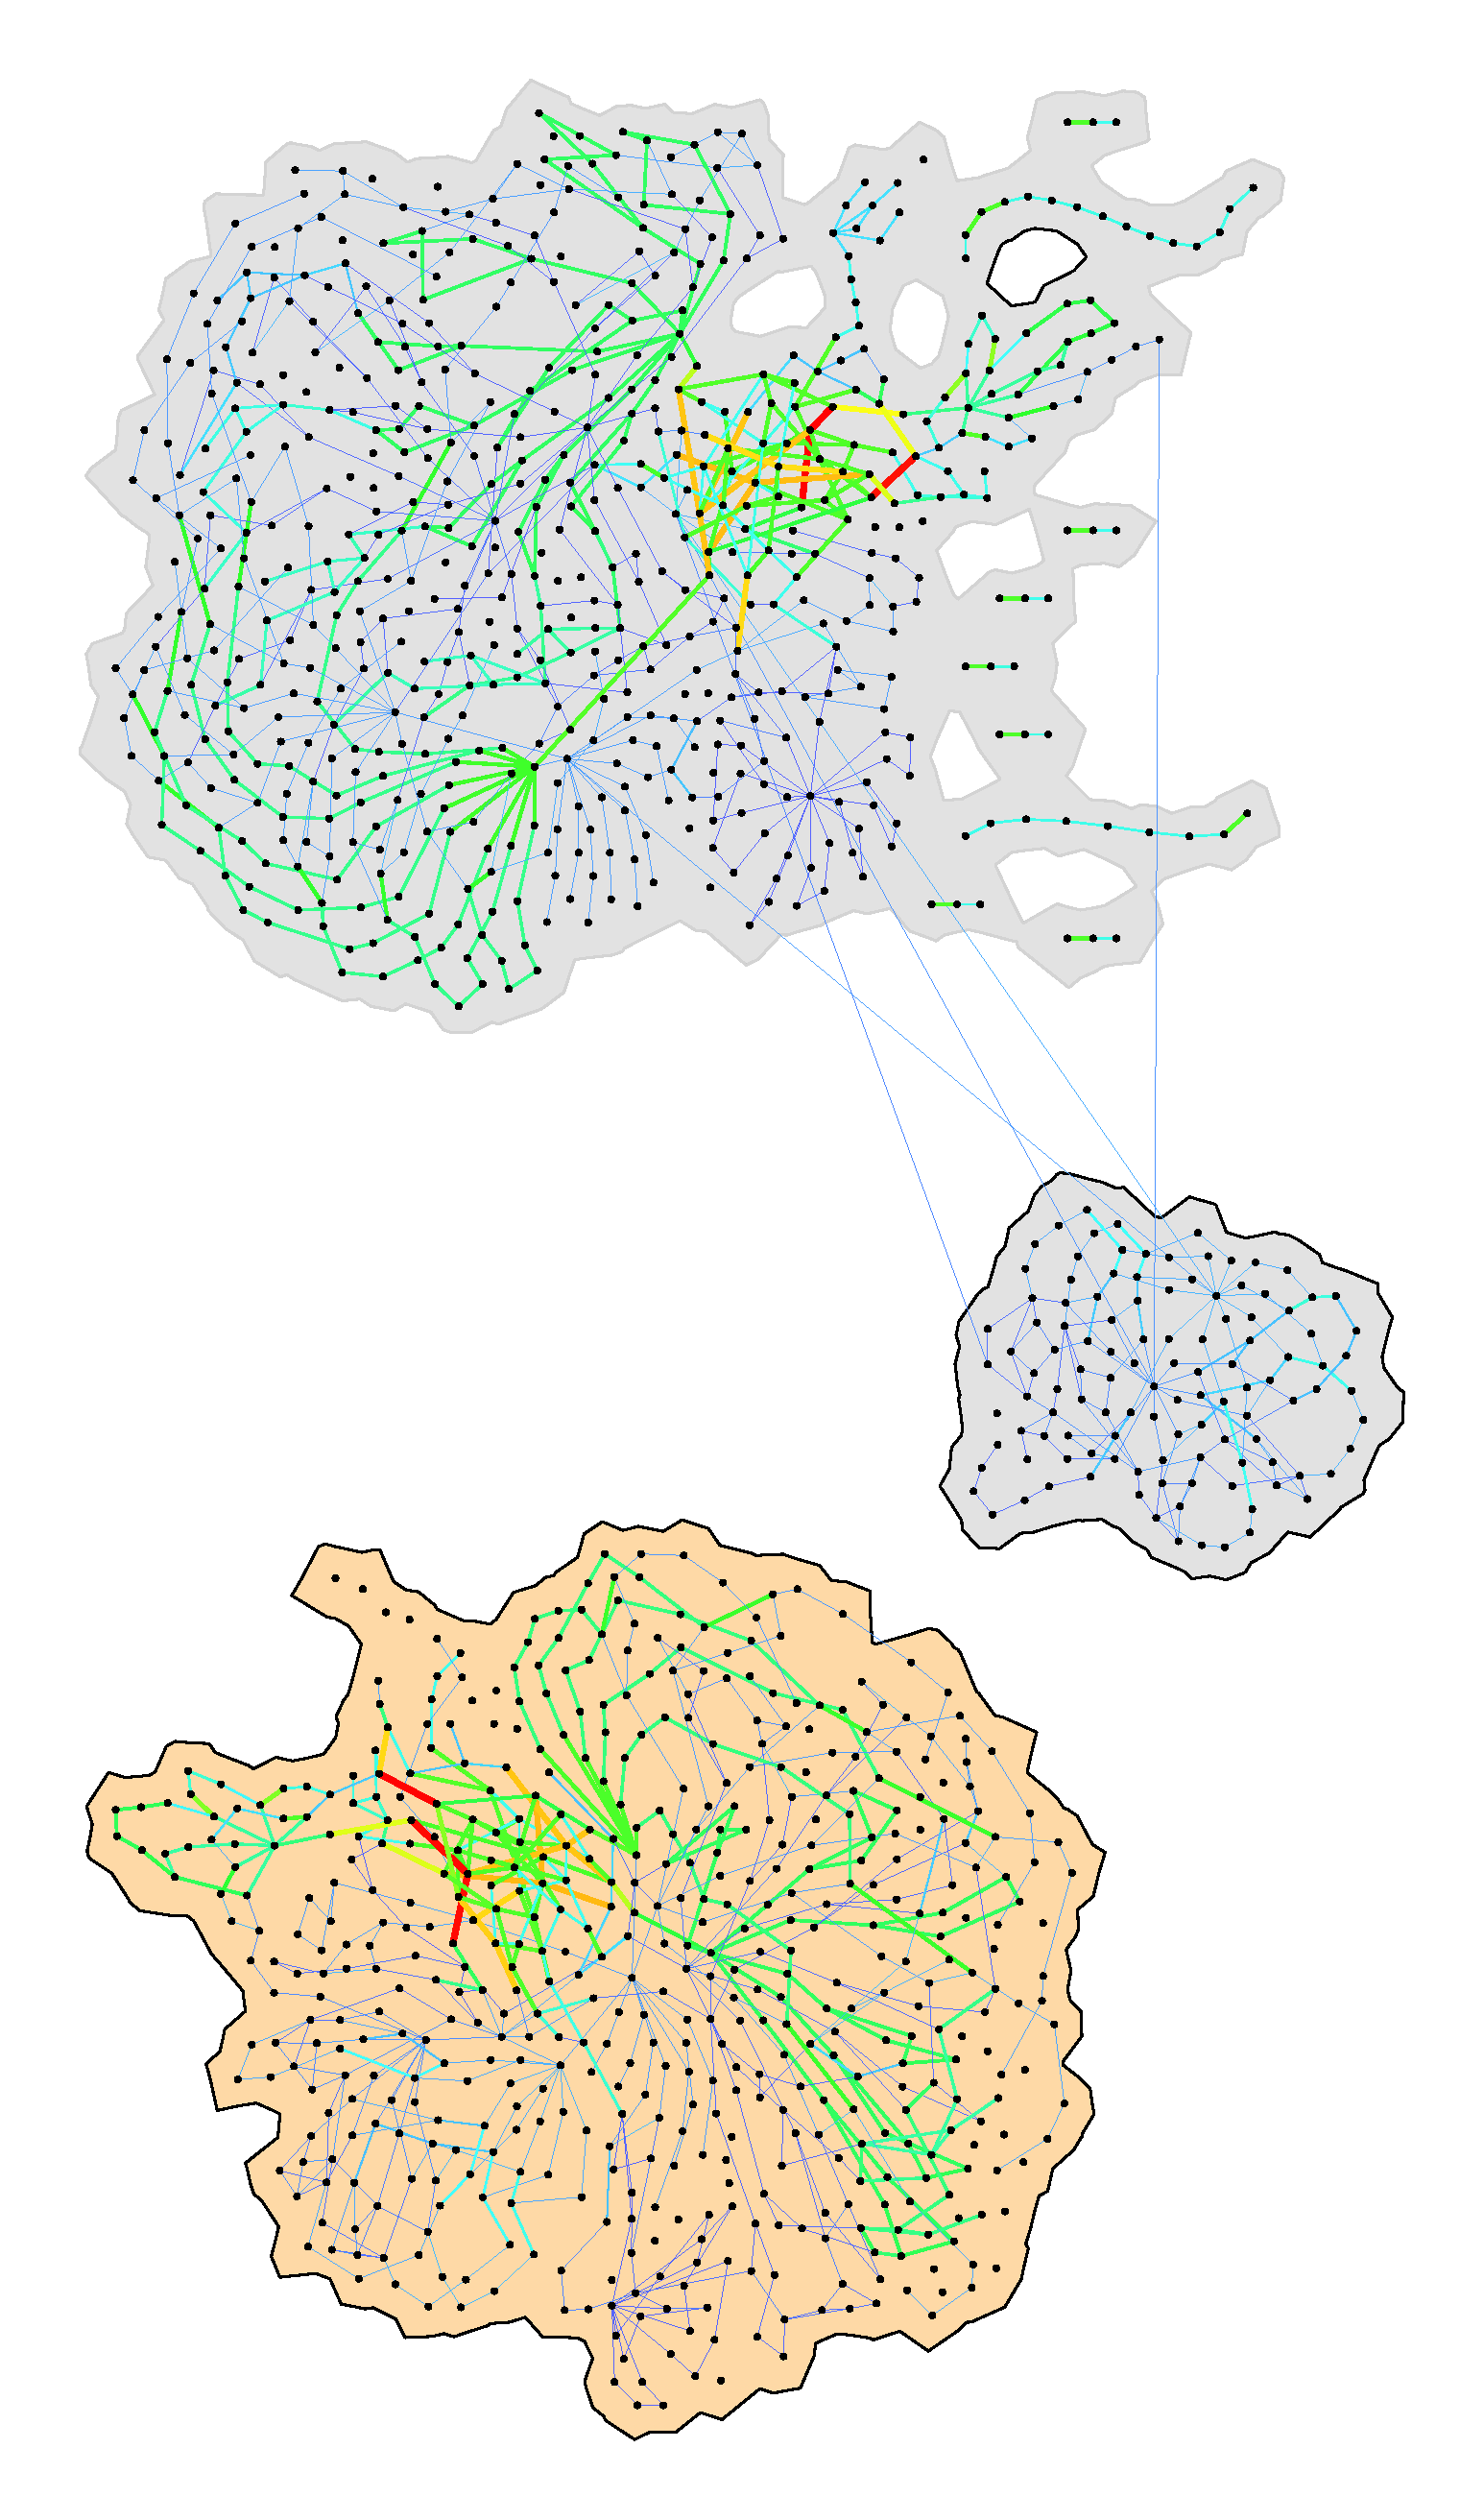
\includegraphics[clip=true,width=0.5\textwidth]{figs/s9234_2part.pdf}
\caption{Heatmap of messages sent during the ISCAS'89 s9234 simulation, partitioned into two partitions using the profile guided algorithm.}
\end{figure}

\begin{figure}
\centering
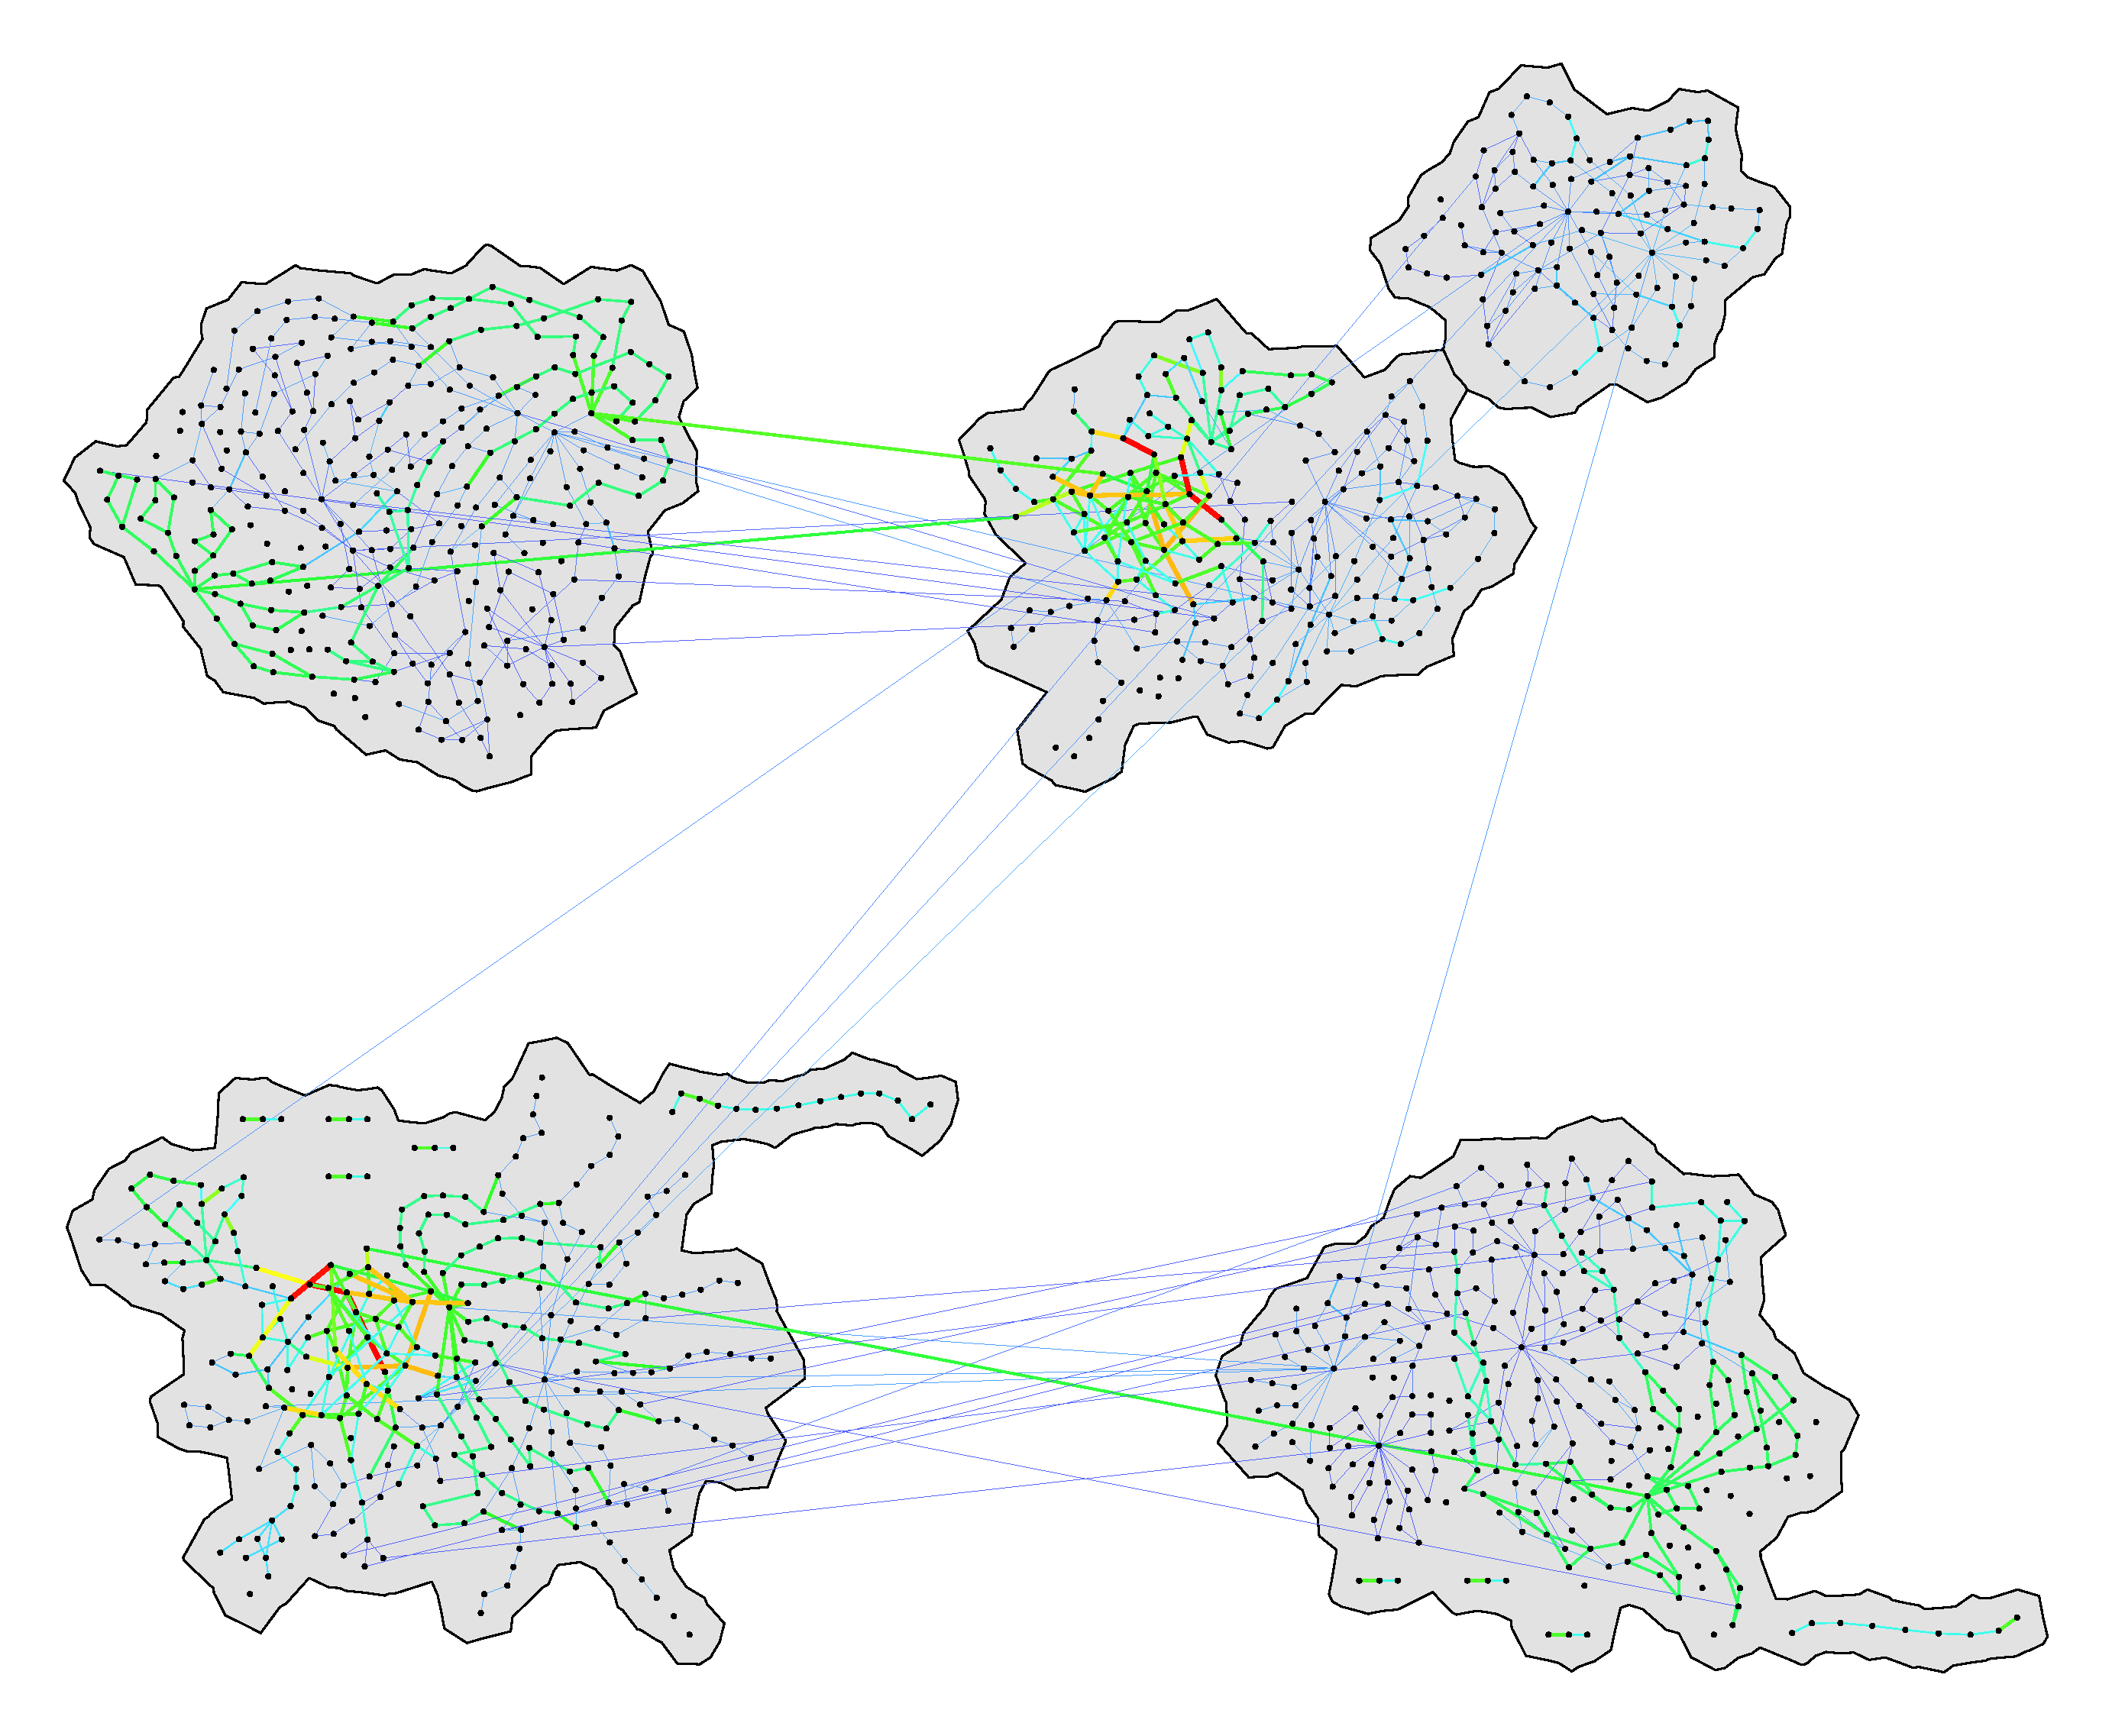
\includegraphics[clip=true,width=0.5\textwidth]{figs/s9234_4part.pdf}
\caption{Heatmap of messages sent during the ISCAS'89 s9234 simulation, partitioned into four partitions using the profile guided algorithm.}
\end{figure}

\begin{figure}
\centering
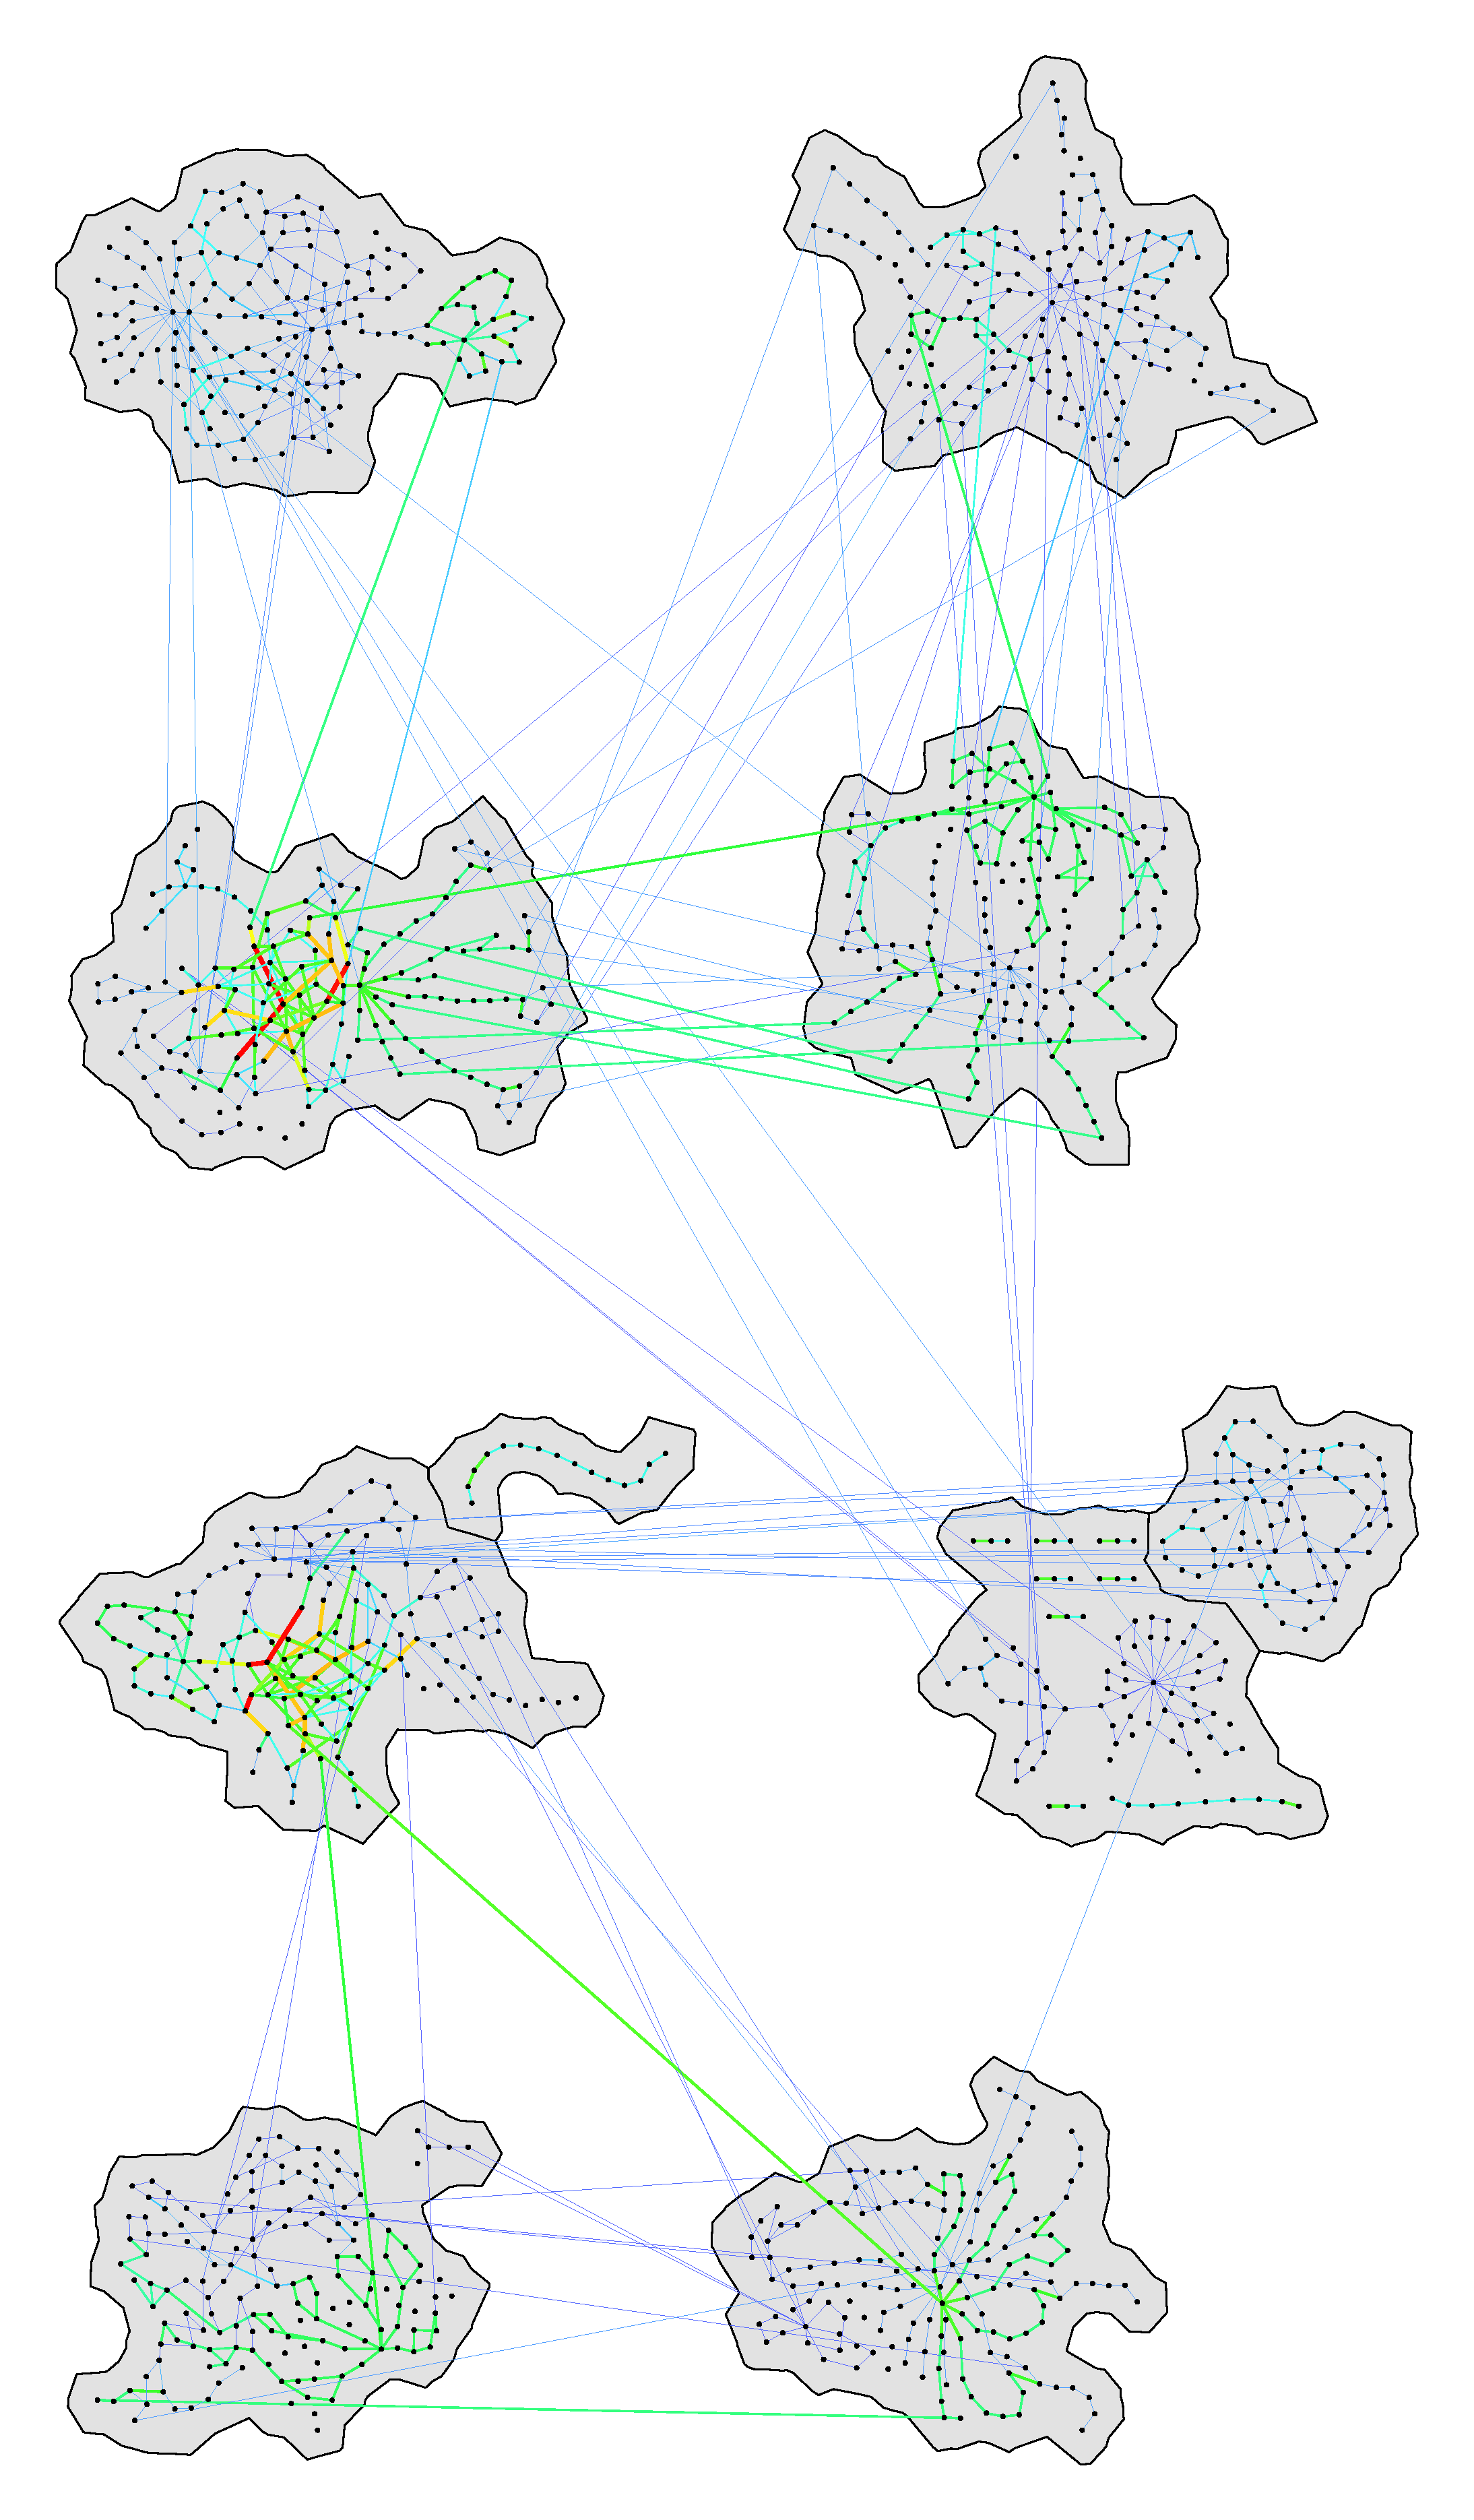
\includegraphics[clip=true,width=0.5\textwidth]{figs/s9234_8part.pdf}
\caption{Heatmap of messages sent during the ISCAS'89 s9234 simulation, partitioned into eight partitions using the profile guided algorithm.}
\end{figure}

\bibliography{refs}
\bibliographystyle{ieeetr} \markright{ }

\end{document}
